% Options for packages loaded elsewhere
\PassOptionsToPackage{unicode}{hyperref}
\PassOptionsToPackage{hyphens}{url}
%
\documentclass[
]{article}
\usepackage{lmodern}
\usepackage{amssymb,amsmath}
\usepackage{ifxetex,ifluatex}
\ifnum 0\ifxetex 1\fi\ifluatex 1\fi=0 % if pdftex
  \usepackage[T1]{fontenc}
  \usepackage[utf8]{inputenc}
  \usepackage{textcomp} % provide euro and other symbols
\else % if luatex or xetex
  \usepackage{unicode-math}
  \defaultfontfeatures{Scale=MatchLowercase}
  \defaultfontfeatures[\rmfamily]{Ligatures=TeX,Scale=1}
\fi
% Use upquote if available, for straight quotes in verbatim environments
\IfFileExists{upquote.sty}{\usepackage{upquote}}{}
\IfFileExists{microtype.sty}{% use microtype if available
  \usepackage[]{microtype}
  \UseMicrotypeSet[protrusion]{basicmath} % disable protrusion for tt fonts
}{}
\makeatletter
\@ifundefined{KOMAClassName}{% if non-KOMA class
  \IfFileExists{parskip.sty}{%
    \usepackage{parskip}
  }{% else
    \setlength{\parindent}{0pt}
    \setlength{\parskip}{6pt plus 2pt minus 1pt}}
}{% if KOMA class
  \KOMAoptions{parskip=half}}
\makeatother
\usepackage{xcolor}
\IfFileExists{xurl.sty}{\usepackage{xurl}}{} % add URL line breaks if available
\IfFileExists{bookmark.sty}{\usepackage{bookmark}}{\usepackage{hyperref}}
\hypersetup{
  pdftitle={Visualization 2: Matching Results},
  pdfauthor={Fan Lu \& Gento Kato},
  hidelinks,
  pdfcreator={LaTeX via pandoc}}
\urlstyle{same} % disable monospaced font for URLs
\usepackage[margin=1in]{geometry}
\usepackage{color}
\usepackage{fancyvrb}
\newcommand{\VerbBar}{|}
\newcommand{\VERB}{\Verb[commandchars=\\\{\}]}
\DefineVerbatimEnvironment{Highlighting}{Verbatim}{commandchars=\\\{\}}
% Add ',fontsize=\small' for more characters per line
\usepackage{framed}
\definecolor{shadecolor}{RGB}{248,248,248}
\newenvironment{Shaded}{\begin{snugshade}}{\end{snugshade}}
\newcommand{\AlertTok}[1]{\textcolor[rgb]{0.94,0.16,0.16}{#1}}
\newcommand{\AnnotationTok}[1]{\textcolor[rgb]{0.56,0.35,0.01}{\textbf{\textit{#1}}}}
\newcommand{\AttributeTok}[1]{\textcolor[rgb]{0.77,0.63,0.00}{#1}}
\newcommand{\BaseNTok}[1]{\textcolor[rgb]{0.00,0.00,0.81}{#1}}
\newcommand{\BuiltInTok}[1]{#1}
\newcommand{\CharTok}[1]{\textcolor[rgb]{0.31,0.60,0.02}{#1}}
\newcommand{\CommentTok}[1]{\textcolor[rgb]{0.56,0.35,0.01}{\textit{#1}}}
\newcommand{\CommentVarTok}[1]{\textcolor[rgb]{0.56,0.35,0.01}{\textbf{\textit{#1}}}}
\newcommand{\ConstantTok}[1]{\textcolor[rgb]{0.00,0.00,0.00}{#1}}
\newcommand{\ControlFlowTok}[1]{\textcolor[rgb]{0.13,0.29,0.53}{\textbf{#1}}}
\newcommand{\DataTypeTok}[1]{\textcolor[rgb]{0.13,0.29,0.53}{#1}}
\newcommand{\DecValTok}[1]{\textcolor[rgb]{0.00,0.00,0.81}{#1}}
\newcommand{\DocumentationTok}[1]{\textcolor[rgb]{0.56,0.35,0.01}{\textbf{\textit{#1}}}}
\newcommand{\ErrorTok}[1]{\textcolor[rgb]{0.64,0.00,0.00}{\textbf{#1}}}
\newcommand{\ExtensionTok}[1]{#1}
\newcommand{\FloatTok}[1]{\textcolor[rgb]{0.00,0.00,0.81}{#1}}
\newcommand{\FunctionTok}[1]{\textcolor[rgb]{0.00,0.00,0.00}{#1}}
\newcommand{\ImportTok}[1]{#1}
\newcommand{\InformationTok}[1]{\textcolor[rgb]{0.56,0.35,0.01}{\textbf{\textit{#1}}}}
\newcommand{\KeywordTok}[1]{\textcolor[rgb]{0.13,0.29,0.53}{\textbf{#1}}}
\newcommand{\NormalTok}[1]{#1}
\newcommand{\OperatorTok}[1]{\textcolor[rgb]{0.81,0.36,0.00}{\textbf{#1}}}
\newcommand{\OtherTok}[1]{\textcolor[rgb]{0.56,0.35,0.01}{#1}}
\newcommand{\PreprocessorTok}[1]{\textcolor[rgb]{0.56,0.35,0.01}{\textit{#1}}}
\newcommand{\RegionMarkerTok}[1]{#1}
\newcommand{\SpecialCharTok}[1]{\textcolor[rgb]{0.00,0.00,0.00}{#1}}
\newcommand{\SpecialStringTok}[1]{\textcolor[rgb]{0.31,0.60,0.02}{#1}}
\newcommand{\StringTok}[1]{\textcolor[rgb]{0.31,0.60,0.02}{#1}}
\newcommand{\VariableTok}[1]{\textcolor[rgb]{0.00,0.00,0.00}{#1}}
\newcommand{\VerbatimStringTok}[1]{\textcolor[rgb]{0.31,0.60,0.02}{#1}}
\newcommand{\WarningTok}[1]{\textcolor[rgb]{0.56,0.35,0.01}{\textbf{\textit{#1}}}}
\usepackage{graphicx,grffile}
\makeatletter
\def\maxwidth{\ifdim\Gin@nat@width>\linewidth\linewidth\else\Gin@nat@width\fi}
\def\maxheight{\ifdim\Gin@nat@height>\textheight\textheight\else\Gin@nat@height\fi}
\makeatother
% Scale images if necessary, so that they will not overflow the page
% margins by default, and it is still possible to overwrite the defaults
% using explicit options in \includegraphics[width, height, ...]{}
\setkeys{Gin}{width=\maxwidth,height=\maxheight,keepaspectratio}
% Set default figure placement to htbp
\makeatletter
\def\fps@figure{htbp}
\makeatother
\setlength{\emergencystretch}{3em} % prevent overfull lines
\providecommand{\tightlist}{%
  \setlength{\itemsep}{0pt}\setlength{\parskip}{0pt}}
\setcounter{secnumdepth}{-\maxdimen} % remove section numbering
\usepackage{bookmark}
\usepackage{xltxtra}
\usepackage{zxjatype}
\usepackage[ipa]{zxjafont}

\title{Visualization 2: Matching Results}
\author{Fan Lu \& Gento Kato}
\date{January 26, 2021}

\begin{document}
\maketitle

\hypertarget{preparation}{%
\section{Preparation}\label{preparation}}

\begin{Shaded}
\begin{Highlighting}[]
\CommentTok{## Clean Up Space}
\KeywordTok{rm}\NormalTok{(}\DataTypeTok{list=}\KeywordTok{ls}\NormalTok{())}

\CommentTok{## Set Working Directory (Automatically) ##}
\KeywordTok{require}\NormalTok{(rstudioapi); }\KeywordTok{require}\NormalTok{(rprojroot)}
\ControlFlowTok{if}\NormalTok{ (rstudioapi}\OperatorTok{::}\KeywordTok{isAvailable}\NormalTok{()}\OperatorTok{==}\OtherTok{TRUE}\NormalTok{) \{}
  \KeywordTok{setwd}\NormalTok{(}\KeywordTok{dirname}\NormalTok{(rstudioapi}\OperatorTok{::}\KeywordTok{getActiveDocumentContext}\NormalTok{()}\OperatorTok{$}\NormalTok{path)); }
\NormalTok{\} }
\NormalTok{projdir <-}\StringTok{ }\KeywordTok{find_root}\NormalTok{(}\KeywordTok{has_file}\NormalTok{(}\StringTok{"thisishome.txt"}\NormalTok{))}
\KeywordTok{cat}\NormalTok{(}\KeywordTok{paste}\NormalTok{(}\StringTok{"Working Directory Set to:}\CharTok{\textbackslash{}n}\StringTok{"}\NormalTok{,projdir))}
\end{Highlighting}
\end{Shaded}

\begin{verbatim}
## Working Directory Set to:
##  /home/gentok/GoogleDrive/Projects/Fan-Gento-Lab/ForeignerJapan
\end{verbatim}

\begin{Shaded}
\begin{Highlighting}[]
\KeywordTok{setwd}\NormalTok{(projdir)}

\CommentTok{## Import Matched Data}

\NormalTok{d <-}\StringTok{ }\KeywordTok{readRDS}\NormalTok{(}\KeywordTok{paste0}\NormalTok{(projdir, }\StringTok{"/data/sifcct_zip_latest_v5.rds"}\NormalTok{))}
\NormalTok{dy <-}\StringTok{ }\KeywordTok{readRDS}\NormalTok{(}\KeywordTok{paste0}\NormalTok{(projdir, }\StringTok{"/data/sifcct_unmatched_v5.rds"}\NormalTok{))}
\NormalTok{dym1 <-}\StringTok{ }\KeywordTok{readRDS}\NormalTok{(}\KeywordTok{paste0}\NormalTok{(projdir, }\StringTok{"/data/sifcct_matched_1_all_v5.rds"}\NormalTok{))}
\NormalTok{dym2 <-}\StringTok{ }\KeywordTok{readRDS}\NormalTok{(}\KeywordTok{paste0}\NormalTok{(projdir, }\StringTok{"/data/sifcct_matched_2_all_v5.rds"}\NormalTok{))}
\NormalTok{dym3 <-}\StringTok{ }\KeywordTok{readRDS}\NormalTok{(}\KeywordTok{paste0}\NormalTok{(projdir, }\StringTok{"/data/sifcct_matched_3_all_v5.rds"}\NormalTok{))}
\NormalTok{dym4 <-}\StringTok{ }\KeywordTok{readRDS}\NormalTok{(}\KeywordTok{paste0}\NormalTok{(projdir, }\StringTok{"/data/sifcct_matched_4_all_v5.rds"}\NormalTok{))}
\NormalTok{dym5 <-}\StringTok{ }\KeywordTok{readRDS}\NormalTok{(}\KeywordTok{paste0}\NormalTok{(projdir, }\StringTok{"/data/sifcct_matched_5_all_v5.rds"}\NormalTok{))}

\CommentTok{## Fix Pair ID }
\NormalTok{updatepairid <-}\StringTok{ }\ControlFlowTok{function}\NormalTok{(dym1) \{}
\NormalTok{  dym1}\OperatorTok{$}\NormalTok{pair_id[}\KeywordTok{which}\NormalTok{(dym1}\OperatorTok{$}\NormalTok{femalebefore}\OperatorTok{==}\DecValTok{1}\NormalTok{)] <-}\StringTok{ }\KeywordTok{paste0}\NormalTok{(}\StringTok{"fb_"}\NormalTok{,dym1}\OperatorTok{$}\NormalTok{pair_id[}\KeywordTok{which}\NormalTok{(dym1}\OperatorTok{$}\NormalTok{femalebefore}\OperatorTok{==}\DecValTok{1}\NormalTok{)]) }
\NormalTok{  dym1}\OperatorTok{$}\NormalTok{pair_id[}\KeywordTok{which}\NormalTok{(dym1}\OperatorTok{$}\NormalTok{femaleafter}\OperatorTok{==}\DecValTok{1}\NormalTok{)] <-}\StringTok{ }\KeywordTok{paste0}\NormalTok{(}\StringTok{"fa_"}\NormalTok{,dym1}\OperatorTok{$}\NormalTok{pair_id[}\KeywordTok{which}\NormalTok{(dym1}\OperatorTok{$}\NormalTok{femaleafter}\OperatorTok{==}\DecValTok{1}\NormalTok{)]) }
\NormalTok{  dym1}\OperatorTok{$}\NormalTok{pair_id[}\KeywordTok{which}\NormalTok{(dym1}\OperatorTok{$}\NormalTok{malebefore}\OperatorTok{==}\DecValTok{1}\NormalTok{)] <-}\StringTok{ }\KeywordTok{paste0}\NormalTok{(}\StringTok{"mb_"}\NormalTok{,dym1}\OperatorTok{$}\NormalTok{pair_id[}\KeywordTok{which}\NormalTok{(dym1}\OperatorTok{$}\NormalTok{malebefore}\OperatorTok{==}\DecValTok{1}\NormalTok{)]) }
\NormalTok{  dym1}\OperatorTok{$}\NormalTok{pair_id[}\KeywordTok{which}\NormalTok{(dym1}\OperatorTok{$}\NormalTok{maleafter}\OperatorTok{==}\DecValTok{1}\NormalTok{)] <-}\StringTok{ }\KeywordTok{paste0}\NormalTok{(}\StringTok{"ma_"}\NormalTok{,dym1}\OperatorTok{$}\NormalTok{pair_id[}\KeywordTok{which}\NormalTok{(dym1}\OperatorTok{$}\NormalTok{maleafter}\OperatorTok{==}\DecValTok{1}\NormalTok{)]) }
  \KeywordTok{return}\NormalTok{(dym1)}
\NormalTok{\}}
\NormalTok{dym1 <-}\StringTok{ }\KeywordTok{updatepairid}\NormalTok{(dym1)}
\NormalTok{dym2 <-}\StringTok{ }\KeywordTok{updatepairid}\NormalTok{(dym2)}
\NormalTok{dym3 <-}\StringTok{ }\KeywordTok{updatepairid}\NormalTok{(dym3)}
\NormalTok{dym4 <-}\StringTok{ }\KeywordTok{updatepairid}\NormalTok{(dym4)}
\NormalTok{dym5 <-}\StringTok{ }\KeywordTok{updatepairid}\NormalTok{(dym5)}

\CommentTok{## Packages}
\KeywordTok{library}\NormalTok{(lmtest) }\CommentTok{# For Statistical Test}
\KeywordTok{library}\NormalTok{(sandwich) }\CommentTok{# Cluster Robust Standard Error}
\KeywordTok{library}\NormalTok{(ggplot2) }\CommentTok{# Plotting }
\KeywordTok{library}\NormalTok{(grid) }\CommentTok{# Plotting  }
\KeywordTok{library}\NormalTok{(gridExtra) }\CommentTok{# Plotting}
\KeywordTok{library}\NormalTok{(sf) }\CommentTok{# Plotting Map}
\KeywordTok{library}\NormalTok{(ggimage) }\CommentTok{# Plotting Map}
\KeywordTok{library}\NormalTok{(jpndistrict) }\CommentTok{# Plotting Japanese Map}
\KeywordTok{library}\NormalTok{(magrittr) }\CommentTok{# Data Management/Plotting}
\KeywordTok{library}\NormalTok{(purrr) }\CommentTok{# Data Management}
\KeywordTok{library}\NormalTok{(pbapply) }\CommentTok{# Apply with Progress Bar}
\KeywordTok{require}\NormalTok{(ebal) }\CommentTok{# Matching Balance}
\KeywordTok{require}\NormalTok{(Matching) }\CommentTok{# Matching Balance}
\end{Highlighting}
\end{Shaded}

\hypertarget{plotting-individual-level-predictors-balance}{%
\section{Plotting Individual-Level Predictors
Balance}\label{plotting-individual-level-predictors-balance}}

\begin{Shaded}
\begin{Highlighting}[]
\CommentTok{## Import Data}
\NormalTok{bal_dy_unmatched <-}\StringTok{ }\KeywordTok{readRDS}\NormalTok{(}\KeywordTok{paste0}\NormalTok{(projdir, }\StringTok{"/data/sifcct_unmatched_balance_v5.rds"}\NormalTok{)) }\CommentTok{# Young, No Distance Adjustment}
\NormalTok{bal_dy_matched_}\DecValTok{1}\NormalTok{ <-}\StringTok{ }\KeywordTok{readRDS}\NormalTok{(}\KeywordTok{paste0}\NormalTok{(projdir, }\StringTok{"/data/sifcct_matched_1_balance_v5.rds"}\NormalTok{)) }\CommentTok{# Young, No Distance Adjustment}
\NormalTok{bal_dy_matched_}\DecValTok{2}\NormalTok{ <-}\StringTok{ }\KeywordTok{readRDS}\NormalTok{(}\KeywordTok{paste0}\NormalTok{(projdir, }\StringTok{"/data/sifcct_matched_2_balance_v5.rds"}\NormalTok{)) }\CommentTok{# Young, Distance Adjusted 50km}
\NormalTok{bal_dy_matched_}\DecValTok{3}\NormalTok{  <-}\StringTok{ }\KeywordTok{readRDS}\NormalTok{(}\KeywordTok{paste0}\NormalTok{(projdir, }\StringTok{"/data/sifcct_matched_3_balance_v5.rds"}\NormalTok{)) }\CommentTok{# Young, Distance Adjusted 100km}
\NormalTok{bal_dy_matched_}\DecValTok{4}\NormalTok{  <-}\StringTok{ }\KeywordTok{readRDS}\NormalTok{(}\KeywordTok{paste0}\NormalTok{(projdir, }\StringTok{"/data/sifcct_matched_4_balance_v5.rds"}\NormalTok{)) }\CommentTok{# Young, Distance Adjusted 200km}
\NormalTok{bal_dy_matched_}\DecValTok{5}\NormalTok{  <-}\StringTok{ }\KeywordTok{readRDS}\NormalTok{(}\KeywordTok{paste0}\NormalTok{(projdir, }\StringTok{"/data/sifcct_matched_5_balance_v5.rds"}\NormalTok{)) }\CommentTok{# Young, Distance Adjusted 350km}

\CommentTok{## Raw data balance}

\CommentTok{## Matching Function}
\KeywordTok{source}\NormalTok{(}\KeywordTok{paste0}\NormalTok{(projdir,}\StringTok{"/src/findmatch.R"}\NormalTok{))}

\NormalTok{fmbal =}\StringTok{ }\KeywordTok{formula}\NormalTok{(edu2 }\OperatorTok{~}\StringTok{ }\NormalTok{female }\OperatorTok{+}\StringTok{ }\NormalTok{age }\OperatorTok{+}\StringTok{ }\NormalTok{bornyr }\OperatorTok{+}\StringTok{ }\NormalTok{lvlen }\OperatorTok{+}\StringTok{ }\NormalTok{lvpr }\OperatorTok{+}\StringTok{ }
\StringTok{                  }\NormalTok{c10_sreg_fper }\OperatorTok{+}\StringTok{ }\KeywordTok{I}\NormalTok{(}\KeywordTok{sqrt}\NormalTok{(c10_sreg_fper)) }\OperatorTok{+}\StringTok{ }\NormalTok{c10_sreg_foreignN }\OperatorTok{+}\StringTok{ }\NormalTok{c10_sreg_pop }\OperatorTok{+}\StringTok{ }
\StringTok{                  }\NormalTok{c10_sreg_edu_ugsP }\OperatorTok{+}\StringTok{ }\NormalTok{c10_sreg_edu_ugs }\OperatorTok{+}\StringTok{ }\NormalTok{c10_sreg_edu_graduated }\OperatorTok{+}\StringTok{ }
\StringTok{                  }\NormalTok{c10_mun_fper }\OperatorTok{+}\StringTok{ }\KeywordTok{I}\NormalTok{(}\KeywordTok{sqrt}\NormalTok{(c10_mun_fper)) }\OperatorTok{+}\StringTok{ }\NormalTok{c10_mun_foreignN }\OperatorTok{+}\StringTok{ }\NormalTok{c10_mun_pop }\OperatorTok{+}\StringTok{ }
\StringTok{                  }\NormalTok{c10_mun_edu_ugsP }\OperatorTok{+}\StringTok{ }\NormalTok{c10_mun_edu_ugs }\OperatorTok{+}\StringTok{ }\NormalTok{c10_mun_edu_graduated }\OperatorTok{+}\StringTok{ }
\StringTok{                  }\NormalTok{zip_did }\OperatorTok{+}\StringTok{ }\NormalTok{didper }\OperatorTok{+}\StringTok{ }\NormalTok{wave }\OperatorTok{+}\StringTok{ }\NormalTok{after }\OperatorTok{+}\StringTok{ }\NormalTok{panel)}
\NormalTok{vnbal =}\StringTok{ }\KeywordTok{c}\NormalTok{(}\StringTok{"Gender"}\NormalTok{,}\StringTok{"Age"}\NormalTok{,}\StringTok{"Born Year"}\NormalTok{,}\StringTok{"Livng Length"}\NormalTok{,}\StringTok{"Living Proportion"}\NormalTok{,}
          \StringTok{"Foreigner Percentage (zip)"}\NormalTok{, }\StringTok{"Foreigner Percentage sqrt. (zip)"}\NormalTok{, }
          \StringTok{"Foreigner Population (zip)"}\NormalTok{, }\StringTok{"Population (zip)"}\NormalTok{,}
          \StringTok{"University Percentage (zip)"}\NormalTok{,  }
          \StringTok{"University Population (zip)"}\NormalTok{, }\StringTok{"Graduated Population (zip)"}\NormalTok{,}
          \StringTok{"Foreigner Percentage (mun.)"}\NormalTok{, }\StringTok{"Foreigner Percentage sqrt. (mun.)"}\NormalTok{, }
          \StringTok{"Foreigner Population (mun.)"}\NormalTok{, }\StringTok{"Population (mun.)"}\NormalTok{,}
          \StringTok{"University Percentage (mun.)"}\NormalTok{,  }
          \StringTok{"University Population (mun.)"}\NormalTok{, }\StringTok{"Graduated Population (mun.)"}\NormalTok{,}
          \StringTok{"DID Residence"}\NormalTok{,}\StringTok{"DID Proportion"}\NormalTok{,}\StringTok{"Wave"}\NormalTok{,}\StringTok{"Aug. 2012 or After"}\NormalTok{,}\StringTok{"Panel"}\NormalTok{)}

\CommentTok{### Female}
\NormalTok{balf_dy_unmatched <-}\StringTok{ }\KeywordTok{findbalance}\NormalTok{(dy[dy}\OperatorTok{$}\NormalTok{female}\OperatorTok{==}\DecValTok{1}\NormalTok{,], fmbal, vnbal)}
\KeywordTok{round}\NormalTok{(balf_dy_unmatched,}\DecValTok{3}\NormalTok{)[,}\DecValTok{1}\OperatorTok{:}\DecValTok{7}\NormalTok{]}
\end{Highlighting}
\end{Shaded}

\begin{verbatim}
##                                      mean.Tr    mean.Co   sdiff sdiff.pooled var.ratio T pval KS pval
## Gender                                 1.000      1.000   0.000        0.000       NaN  1.000      NA
## Age                                   35.614     44.297 -68.600      -67.072     0.916  0.000   0.000
## Born Year                           1976.308   1967.666  68.299       66.794     0.916  0.000   0.000
## Livng Length                          31.581     41.358 -70.775      -69.669     0.940  0.000   0.000
## Living Proportion                      0.870      0.924 -32.565      -36.994     1.819  0.000   0.000
## Foreigner Percentage (zip)             1.487      1.332   4.831        5.651     2.167  0.130   0.000
## Foreigner Percentage sqrt. (zip)       1.038      0.955  12.966       12.880     0.974  0.000   0.000
## Foreigner Population (zip)           127.311     92.861  12.784       14.230     1.629  0.000   0.000
## Population (zip)                    6898.757   5559.082  18.482       19.867     1.368  0.000   0.000
## University Percentage (zip)           21.319     17.098  46.515       48.944     1.240  0.000   0.000
## University Population (zip)         1320.148    858.543  27.479       31.602     1.952  0.000   0.000
## Graduated Population (zip)          5489.361   4428.532  18.265       19.646     1.373  0.000   0.000
## Foreigner Percentage (mun.)            1.447      1.279  13.905       12.678     0.711  0.000   0.000
## Foreigner Percentage sqrt. (mun.)      1.124      1.028  22.181       21.143     0.832  0.000   0.000
## Foreigner Population (mun.)         3644.498   2976.128  15.311       15.792     1.136  0.000   0.000
## Population (mun.)                 238367.915 217214.812  11.825       12.246     1.156  0.001   0.006
## University Percentage (mun.)          19.910     16.898  44.492       45.851     1.132  0.000   0.000
## University Population (mun.)       40337.562  32009.598  22.331       24.394     1.479  0.000   0.000
## Graduated Population (mun.)       189577.702 172755.826  11.767       12.236     1.177  0.001   0.008
## DID Residence                          0.738      0.677  13.967       13.530     0.884  0.000      NA
## DID Proportion                         0.781      0.704  28.269       26.907     0.828  0.000   0.000
## Wave                                  11.649     12.030  -6.024       -6.133     1.076  0.093   0.030
## Aug. 2012 or After                     0.545      0.576  -6.286       -6.310     1.016  0.083      NA
## Panel                                  0.047      0.052  -2.203       -2.153     0.914  0.552      NA
\end{verbatim}

\begin{Shaded}
\begin{Highlighting}[]
\CommentTok{### Male}
\NormalTok{balm_dy_unmatched <-}\StringTok{ }\KeywordTok{findbalance}\NormalTok{(dy[dy}\OperatorTok{$}\NormalTok{male}\OperatorTok{==}\DecValTok{1}\NormalTok{,], fmbal, vnbal)}
\KeywordTok{round}\NormalTok{(balm_dy_unmatched,}\DecValTok{3}\NormalTok{)[,}\DecValTok{1}\OperatorTok{:}\DecValTok{7}\NormalTok{]}
\end{Highlighting}
\end{Shaded}

\begin{verbatim}
##                                      mean.Tr    mean.Co   sdiff sdiff.pooled var.ratio T pval KS pval
## Gender                                 0.000      0.000   0.000        0.000       NaN  1.000      NA
## Age                                   44.016     45.479 -10.370      -10.580     1.085  0.000    0.00
## Born Year                           1967.901   1966.461  10.195       10.396     1.083  0.001    0.00
## Livng Length                          40.305     42.622 -15.328      -15.653     1.089  0.000    0.00
## Living Proportion                      0.902      0.928 -19.177      -20.225     1.253  0.000    0.00
## Foreigner Percentage (zip)             1.357      1.126  12.843       14.015     1.472  0.000    0.00
## Foreigner Percentage sqrt. (zip)       1.006      0.898  18.348       18.704     1.082  0.000    0.00
## Foreigner Population (zip)           106.053     71.883  15.496       17.307     1.657  0.000    0.00
## Population (zip)                    6393.051   4935.819  21.400       23.130     1.405  0.000    0.00
## University Percentage (zip)           19.695     15.798  45.201       47.934     1.285  0.000    0.00
## University Population (zip)         1161.691    724.864  28.244       32.963     2.135  0.000    0.00
## Graduated Population (zip)          5101.522   3942.693  21.242       22.959     1.405  0.000    0.00
## Foreigner Percentage (mun.)            1.405      1.174  17.590       19.557     1.619  0.000    0.00
## Foreigner Percentage sqrt. (mun.)      1.103      1.002  23.025       23.656     1.118  0.000    0.00
## Foreigner Population (mun.)         3482.812   2456.075  24.170       27.236     1.739  0.000    0.00
## Population (mun.)                 234059.670 190426.378  23.929       25.812     1.391  0.000    0.00
## University Percentage (mun.)          18.965     16.032  43.664       45.625     1.202  0.000    0.00
## University Population (mun.)       38297.775  27569.190  29.116       32.893     1.763  0.000    0.00
## Graduated Population (mun.)       186083.053 151516.953  23.831       25.785     1.412  0.000    0.00
## DID Residence                          0.713      0.591  26.963       25.820     0.847  0.000      NA
## DID Proportion                         0.747      0.635  38.766       36.383     0.787  0.000    0.00
## Wave                                  11.670     11.755  -1.389       -1.404     1.045  0.639    0.19
## Aug. 2012 or After                     0.557      0.562  -0.937       -0.938     1.002  0.755      NA
## Panel                                  0.050      0.052  -1.169       -1.155     0.954  0.701      NA
\end{verbatim}

\begin{Shaded}
\begin{Highlighting}[]
\CommentTok{## Matched Sample Proportions}
\NormalTok{matchprdt <-}\StringTok{ }\KeywordTok{data.frame}\NormalTok{(}
  \DataTypeTok{labs =} \KeywordTok{c}\NormalTok{(}\StringTok{"Unmatched"}\NormalTok{,}
           \StringTok{"Matched without Distance Adjustment"}\NormalTok{,}
           \StringTok{"Matched with Lambda = 350km"}\NormalTok{,}
           \StringTok{"Matched with Lambda = 200km"}\NormalTok{,}
           \StringTok{"Matched with Lambda = 100km"}\NormalTok{,}
           \StringTok{"Matched with Lambda = 50km"}\NormalTok{),}
  \DataTypeTok{notF =} \KeywordTok{c}\NormalTok{(}\KeywordTok{table}\NormalTok{(dy[dy}\OperatorTok{$}\NormalTok{female}\OperatorTok{==}\DecValTok{1}\NormalTok{,]}\OperatorTok{$}\NormalTok{edu2)[}\DecValTok{1}\NormalTok{],}
           \KeywordTok{table}\NormalTok{(dym1[dym1}\OperatorTok{$}\NormalTok{female}\OperatorTok{==}\DecValTok{1}\NormalTok{,]}\OperatorTok{$}\NormalTok{edu2)[}\DecValTok{1}\NormalTok{],}
           \KeywordTok{table}\NormalTok{(dym5[dym5}\OperatorTok{$}\NormalTok{female}\OperatorTok{==}\DecValTok{1}\NormalTok{,]}\OperatorTok{$}\NormalTok{edu2)[}\DecValTok{1}\NormalTok{],}
           \KeywordTok{table}\NormalTok{(dym4[dym4}\OperatorTok{$}\NormalTok{female}\OperatorTok{==}\DecValTok{1}\NormalTok{,]}\OperatorTok{$}\NormalTok{edu2)[}\DecValTok{1}\NormalTok{],}
           \KeywordTok{table}\NormalTok{(dym3[dym3}\OperatorTok{$}\NormalTok{female}\OperatorTok{==}\DecValTok{1}\NormalTok{,]}\OperatorTok{$}\NormalTok{edu2)[}\DecValTok{1}\NormalTok{],}
           \KeywordTok{table}\NormalTok{(dym2[dym2}\OperatorTok{$}\NormalTok{female}\OperatorTok{==}\DecValTok{1}\NormalTok{,]}\OperatorTok{$}\NormalTok{edu2)[}\DecValTok{1}\NormalTok{]),}
  \DataTypeTok{treatedF =} \KeywordTok{c}\NormalTok{(}\KeywordTok{table}\NormalTok{(dy[dy}\OperatorTok{$}\NormalTok{female}\OperatorTok{==}\DecValTok{1}\NormalTok{,]}\OperatorTok{$}\NormalTok{edu2)[}\DecValTok{2}\NormalTok{],}
               \KeywordTok{table}\NormalTok{(dym1[dym1}\OperatorTok{$}\NormalTok{female}\OperatorTok{==}\DecValTok{1}\NormalTok{,]}\OperatorTok{$}\NormalTok{edu2)[}\DecValTok{2}\NormalTok{],}
               \KeywordTok{table}\NormalTok{(dym5[dym5}\OperatorTok{$}\NormalTok{female}\OperatorTok{==}\DecValTok{1}\NormalTok{,]}\OperatorTok{$}\NormalTok{edu2)[}\DecValTok{2}\NormalTok{],}
               \KeywordTok{table}\NormalTok{(dym4[dym4}\OperatorTok{$}\NormalTok{female}\OperatorTok{==}\DecValTok{1}\NormalTok{,]}\OperatorTok{$}\NormalTok{edu2)[}\DecValTok{2}\NormalTok{],}
               \KeywordTok{table}\NormalTok{(dym3[dym3}\OperatorTok{$}\NormalTok{female}\OperatorTok{==}\DecValTok{1}\NormalTok{,]}\OperatorTok{$}\NormalTok{edu2)[}\DecValTok{2}\NormalTok{],}
               \KeywordTok{table}\NormalTok{(dym2[dym2}\OperatorTok{$}\NormalTok{female}\OperatorTok{==}\DecValTok{1}\NormalTok{,]}\OperatorTok{$}\NormalTok{edu2)[}\DecValTok{2}\NormalTok{]), }
  \DataTypeTok{notM =} \KeywordTok{c}\NormalTok{(}\KeywordTok{table}\NormalTok{(dy[dy}\OperatorTok{$}\NormalTok{female}\OperatorTok{==}\DecValTok{0}\NormalTok{,]}\OperatorTok{$}\NormalTok{edu2)[}\DecValTok{1}\NormalTok{],}
           \KeywordTok{table}\NormalTok{(dym1[dym1}\OperatorTok{$}\NormalTok{female}\OperatorTok{==}\DecValTok{0}\NormalTok{,]}\OperatorTok{$}\NormalTok{edu2)[}\DecValTok{1}\NormalTok{],}
           \KeywordTok{table}\NormalTok{(dym5[dym5}\OperatorTok{$}\NormalTok{female}\OperatorTok{==}\DecValTok{0}\NormalTok{,]}\OperatorTok{$}\NormalTok{edu2)[}\DecValTok{1}\NormalTok{],}
           \KeywordTok{table}\NormalTok{(dym4[dym4}\OperatorTok{$}\NormalTok{female}\OperatorTok{==}\DecValTok{0}\NormalTok{,]}\OperatorTok{$}\NormalTok{edu2)[}\DecValTok{1}\NormalTok{],}
           \KeywordTok{table}\NormalTok{(dym3[dym3}\OperatorTok{$}\NormalTok{female}\OperatorTok{==}\DecValTok{0}\NormalTok{,]}\OperatorTok{$}\NormalTok{edu2)[}\DecValTok{1}\NormalTok{],}
           \KeywordTok{table}\NormalTok{(dym2[dym2}\OperatorTok{$}\NormalTok{female}\OperatorTok{==}\DecValTok{0}\NormalTok{,]}\OperatorTok{$}\NormalTok{edu2)[}\DecValTok{1}\NormalTok{]),  }
  \DataTypeTok{treatedM =} \KeywordTok{c}\NormalTok{(}\KeywordTok{table}\NormalTok{(dy[dy}\OperatorTok{$}\NormalTok{female}\OperatorTok{==}\DecValTok{0}\NormalTok{,]}\OperatorTok{$}\NormalTok{edu2)[}\DecValTok{2}\NormalTok{],}
               \KeywordTok{table}\NormalTok{(dym1[dym1}\OperatorTok{$}\NormalTok{female}\OperatorTok{==}\DecValTok{0}\NormalTok{,]}\OperatorTok{$}\NormalTok{edu2)[}\DecValTok{2}\NormalTok{],}
               \KeywordTok{table}\NormalTok{(dym5[dym5}\OperatorTok{$}\NormalTok{female}\OperatorTok{==}\DecValTok{0}\NormalTok{,]}\OperatorTok{$}\NormalTok{edu2)[}\DecValTok{2}\NormalTok{],}
               \KeywordTok{table}\NormalTok{(dym4[dym4}\OperatorTok{$}\NormalTok{female}\OperatorTok{==}\DecValTok{0}\NormalTok{,]}\OperatorTok{$}\NormalTok{edu2)[}\DecValTok{2}\NormalTok{],}
               \KeywordTok{table}\NormalTok{(dym3[dym3}\OperatorTok{$}\NormalTok{female}\OperatorTok{==}\DecValTok{0}\NormalTok{,]}\OperatorTok{$}\NormalTok{edu2)[}\DecValTok{2}\NormalTok{],}
               \KeywordTok{table}\NormalTok{(dym2[dym2}\OperatorTok{$}\NormalTok{female}\OperatorTok{==}\DecValTok{0}\NormalTok{,]}\OperatorTok{$}\NormalTok{edu2)[}\DecValTok{2}\NormalTok{]))}
\NormalTok{matchprdt}\OperatorTok{$}\NormalTok{prF <-}\StringTok{ }\KeywordTok{round}\NormalTok{((matchprdt}\OperatorTok{$}\NormalTok{notF}\OperatorTok{/}\KeywordTok{table}\NormalTok{(dy[dy}\OperatorTok{$}\NormalTok{female}\OperatorTok{==}\DecValTok{1}\NormalTok{,]}\OperatorTok{$}\NormalTok{edu2)[}\DecValTok{2}\NormalTok{])}\OperatorTok{*}\DecValTok{100}\NormalTok{,}\DecValTok{1}\NormalTok{)}
\NormalTok{matchprdt}\OperatorTok{$}\NormalTok{prM <-}\StringTok{ }\KeywordTok{round}\NormalTok{((matchprdt}\OperatorTok{$}\NormalTok{notM}\OperatorTok{/}\KeywordTok{table}\NormalTok{(dy[dy}\OperatorTok{$}\NormalTok{female}\OperatorTok{==}\DecValTok{0}\NormalTok{,]}\OperatorTok{$}\NormalTok{edu2)[}\DecValTok{1}\NormalTok{])}\OperatorTok{*}\DecValTok{100}\NormalTok{,}\DecValTok{1}\NormalTok{)}
\NormalTok{matchprdt <-}\StringTok{ }\NormalTok{matchprdt[,}\KeywordTok{c}\NormalTok{(}\StringTok{"labs"}\NormalTok{,}\StringTok{"notF"}\NormalTok{,}\StringTok{"treatedF"}\NormalTok{,}\StringTok{"prF"}\NormalTok{,}\StringTok{"notM"}\NormalTok{,}\StringTok{"treatedM"}\NormalTok{,}\StringTok{"prM"}\NormalTok{)]}

\NormalTok{matchprdt <-}\StringTok{ }\KeywordTok{as.matrix}\NormalTok{(matchprdt)}
\KeywordTok{colnames}\NormalTok{(matchprdt) <-}\StringTok{ }\KeywordTok{c}\NormalTok{(}\StringTok{""}\NormalTok{, }\StringTok{"No Univ."}\NormalTok{, }\StringTok{"Univ."}\NormalTok{, }\StringTok{"% Matched"}\NormalTok{, }
                         \StringTok{"No Univ."}\NormalTok{, }\StringTok{"Univ."}\NormalTok{, }\StringTok{"% Matched"}\NormalTok{)}

\CommentTok{### Table of Data Sizes}
\KeywordTok{require}\NormalTok{(knitr)}
\KeywordTok{require}\NormalTok{(kableExtra)}
\NormalTok{tmp <-}\StringTok{ }\KeywordTok{add_header_above}\NormalTok{(}\KeywordTok{kable}\NormalTok{(matchprdt,}\StringTok{"latex"}\NormalTok{, }\DataTypeTok{booktabs =} \OtherTok{TRUE}\NormalTok{, }\DataTypeTok{linesep =} \StringTok{""}\NormalTok{), }
                        \KeywordTok{c}\NormalTok{(}\StringTok{" "}\NormalTok{, }\StringTok{"Female"}\NormalTok{=}\DecValTok{3}\NormalTok{, }\StringTok{"Male"}\NormalTok{=}\DecValTok{3}\NormalTok{))}
\KeywordTok{cat}\NormalTok{(tmp)}
\end{Highlighting}
\end{Shaded}

\begin{verbatim}
## 
## \begin{tabular}{lllllll}
## \toprule
## \multicolumn{1}{c}{ } & \multicolumn{3}{c}{Female} & \multicolumn{3}{c}{Male} \\
## \cmidrule(l{3pt}r{3pt}){2-4} \cmidrule(l{3pt}r{3pt}){5-7}
##  & No Univ. & Univ. & \% Matched & No Univ. & Univ. & \% Matched\\
## \midrule
## Unmatched & 1778 & 1317 & 135.0 & 1778 & 2954 & 100.0\\
## Matched without Distance Adjustment & 856 & 856 & 65.0 & 1451 & 1451 & 81.6\\
## Matched with Lambda = 350km & 785 & 785 & 59.6 & 1355 & 1355 & 76.2\\
## Matched with Lambda = 200km & 692 & 692 & 52.5 & 1201 & 1201 & 67.5\\
## Matched with Lambda = 100km & 530 & 530 & 40.2 & 934 & 934 & 52.5\\
## Matched with Lambda = 50km & 406 & 406 & 30.8 & 655 & 655 & 36.8\\
## \bottomrule
## \end{tabular}
\end{verbatim}

\begin{Shaded}
\begin{Highlighting}[]
\KeywordTok{writeLines}\NormalTok{(tmp, }\KeywordTok{paste0}\NormalTok{(projdir, }\StringTok{"/out/matchedsizes.tex"}\NormalTok{))}

\CommentTok{### Balance Data}
\NormalTok{baldt <-}\StringTok{ }\KeywordTok{as.data.frame}\NormalTok{(}\KeywordTok{rbind}\NormalTok{(balf_dy_unmatched,}
\NormalTok{               bal_dy_matched_}\DecValTok{1}\OperatorTok{$}\NormalTok{f,}
\NormalTok{               bal_dy_matched_}\DecValTok{5}\OperatorTok{$}\NormalTok{f,}
\NormalTok{               bal_dy_matched_}\DecValTok{4}\OperatorTok{$}\NormalTok{f,}
\NormalTok{               bal_dy_matched_}\DecValTok{3}\OperatorTok{$}\NormalTok{f,}
\NormalTok{               bal_dy_matched_}\DecValTok{2}\OperatorTok{$}\NormalTok{f,}
\NormalTok{               balm_dy_unmatched,}
\NormalTok{               bal_dy_matched_}\DecValTok{1}\OperatorTok{$}\NormalTok{m,}
\NormalTok{               bal_dy_matched_}\DecValTok{5}\OperatorTok{$}\NormalTok{m,}
\NormalTok{               bal_dy_matched_}\DecValTok{4}\OperatorTok{$}\NormalTok{m,}
\NormalTok{               bal_dy_matched_}\DecValTok{3}\OperatorTok{$}\NormalTok{m,}
\NormalTok{               bal_dy_matched_}\DecValTok{2}\OperatorTok{$}\NormalTok{m))}
\NormalTok{baldt <-}\StringTok{ }\KeywordTok{data.frame}\NormalTok{(}\DataTypeTok{stat =} \KeywordTok{c}\NormalTok{(baldt}\OperatorTok{$}\NormalTok{sdiff,baldt}\OperatorTok{$}\StringTok{`}\DataTypeTok{T pval}\StringTok{`}\NormalTok{))}
\NormalTok{baldt}\OperatorTok{$}\NormalTok{data <-}\StringTok{ }\KeywordTok{rep}\NormalTok{(}\KeywordTok{c}\NormalTok{(}\StringTok{"Unmatched"}\NormalTok{,}
                \StringTok{"Matched without Distance Adjustment"}\NormalTok{,}
                \StringTok{"Matched with Lambda = 350km"}\NormalTok{,}
                \StringTok{"Matched with Lambda = 200km"}\NormalTok{,}
                \StringTok{"Matched with Lambda = 100km"}\NormalTok{,}
                \StringTok{"Matched with Lambda = 50km"}\NormalTok{), }\DataTypeTok{each=}\KeywordTok{nrow}\NormalTok{(balf_dy_unmatched))}
\NormalTok{baldt}\OperatorTok{$}\NormalTok{data <-}\StringTok{ }\KeywordTok{factor}\NormalTok{(baldt}\OperatorTok{$}\NormalTok{data, }\DataTypeTok{levels=}\KeywordTok{unique}\NormalTok{(baldt}\OperatorTok{$}\NormalTok{data))}
\NormalTok{baldt}\OperatorTok{$}\NormalTok{vn <-}\StringTok{ }\KeywordTok{factor}\NormalTok{(}\KeywordTok{rownames}\NormalTok{(balf_dy_unmatched), }
                   \DataTypeTok{levels=}\KeywordTok{rev}\NormalTok{(}\KeywordTok{rownames}\NormalTok{(balf_dy_unmatched)))}
\NormalTok{baldt}\OperatorTok{$}\NormalTok{stat_cat <-}\StringTok{ }\KeywordTok{rep}\NormalTok{(}\KeywordTok{c}\NormalTok{(}\StringTok{"Standardized Difference in Means"}\NormalTok{,}
                        \StringTok{"p-value: Difference of Means Test"}\NormalTok{),}
                      \DataTypeTok{each =} \KeywordTok{nrow}\NormalTok{(balf_dy_unmatched)}\OperatorTok{*}\DecValTok{12}\NormalTok{)}
\NormalTok{baldt}\OperatorTok{$}\NormalTok{stat_cat <-}\StringTok{ }\KeywordTok{factor}\NormalTok{(baldt}\OperatorTok{$}\NormalTok{stat_cat, }\DataTypeTok{levels=}\KeywordTok{unique}\NormalTok{(baldt}\OperatorTok{$}\NormalTok{stat_cat))}
\NormalTok{baldt}\OperatorTok{$}\NormalTok{gender <-}\StringTok{ }\KeywordTok{rep}\NormalTok{(}\KeywordTok{c}\NormalTok{(}\StringTok{"Female"}\NormalTok{,}\StringTok{"Male"}\NormalTok{), }\DataTypeTok{each=}\KeywordTok{nrow}\NormalTok{(balf_dy_unmatched)}\OperatorTok{*}\DecValTok{6}\NormalTok{)}
\NormalTok{baldt}\OperatorTok{$}\NormalTok{gender <-}\StringTok{ }\KeywordTok{factor}\NormalTok{(baldt}\OperatorTok{$}\NormalTok{gender, }\DataTypeTok{levels=}\KeywordTok{unique}\NormalTok{(baldt}\OperatorTok{$}\NormalTok{gender))}


\KeywordTok{require}\NormalTok{(ggplot2)}
\NormalTok{p <-}\StringTok{ }\KeywordTok{ggplot}\NormalTok{(baldt, }\KeywordTok{aes}\NormalTok{(}\DataTypeTok{x=}\NormalTok{vn,}\DataTypeTok{y=}\NormalTok{stat)) }\OperatorTok{+}\StringTok{ }
\StringTok{  }\KeywordTok{geom_hline}\NormalTok{(}\KeywordTok{aes}\NormalTok{(}\DataTypeTok{yintercept=}\DecValTok{0}\NormalTok{), }\DataTypeTok{size=}\FloatTok{0.25}\NormalTok{, }\DataTypeTok{linetype=}\DecValTok{1}\NormalTok{) }\OperatorTok{+}\StringTok{ }
\StringTok{  }\KeywordTok{geom_point}\NormalTok{(}\KeywordTok{aes}\NormalTok{(}\DataTypeTok{alpha=}\NormalTok{gender, }\DataTypeTok{shape=}\NormalTok{data), }\DataTypeTok{color=}\StringTok{"black"}\NormalTok{,}
             \DataTypeTok{position=}\KeywordTok{position_dodge}\NormalTok{(}\DataTypeTok{width=}\OperatorTok{-}\FloatTok{0.5}\NormalTok{), }\DataTypeTok{size=}\DecValTok{2}\NormalTok{) }\OperatorTok{+}\StringTok{ }
\StringTok{  }\KeywordTok{facet_grid}\NormalTok{( }\OperatorTok{~}\StringTok{ }\NormalTok{stat_cat, }\DataTypeTok{scales=}\StringTok{"free_x"}\NormalTok{, }\DataTypeTok{switch=}\StringTok{"x"}\NormalTok{) }\OperatorTok{+}\StringTok{ }
\StringTok{  }\KeywordTok{scale_shape_discrete}\NormalTok{(}\DataTypeTok{name=}\StringTok{"Matching}\CharTok{\textbackslash{}n}\StringTok{Status"}\NormalTok{, }
                       \DataTypeTok{labels =} \KeywordTok{c}\NormalTok{(}\StringTok{"Unmatched"}\NormalTok{,}
                                  \StringTok{"Matched without Distance Adjustment"}\NormalTok{,}
                                  \KeywordTok{bquote}\NormalTok{(}\StringTok{"Matched with"}\OperatorTok{~}\NormalTok{lambda}\OperatorTok{~}\StringTok{"= 350km"}\NormalTok{),}
                                  \KeywordTok{bquote}\NormalTok{(}\StringTok{"Matched with"}\OperatorTok{~}\NormalTok{lambda}\OperatorTok{~}\StringTok{"= 200km"}\NormalTok{),}
                                  \KeywordTok{bquote}\NormalTok{(}\StringTok{"Matched with"}\OperatorTok{~}\NormalTok{lambda}\OperatorTok{~}\StringTok{"= 100km"}\NormalTok{),}
                                  \KeywordTok{bquote}\NormalTok{(}\StringTok{"Matched with"}\OperatorTok{~}\NormalTok{lambda}\OperatorTok{~}\StringTok{"= 50km"}\NormalTok{))) }\OperatorTok{+}\StringTok{ }
\StringTok{  }\KeywordTok{scale_alpha_manual}\NormalTok{(}\DataTypeTok{name=}\StringTok{"Gender"}\NormalTok{, }\DataTypeTok{values=}\KeywordTok{c}\NormalTok{(}\StringTok{"Female"}\NormalTok{=}\DecValTok{1}\NormalTok{,}\StringTok{"Male"}\NormalTok{=}\FloatTok{0.5}\NormalTok{)) }\OperatorTok{+}\StringTok{ }
\StringTok{  }\KeywordTok{coord_flip}\NormalTok{() }\OperatorTok{+}
\StringTok{  }\KeywordTok{ylab}\NormalTok{(}\OtherTok{NULL}\NormalTok{) }\OperatorTok{+}\StringTok{ }\KeywordTok{xlab}\NormalTok{(}\OtherTok{NULL}\NormalTok{) }\OperatorTok{+}\StringTok{ }
\StringTok{  }\KeywordTok{guides}\NormalTok{(}\DataTypeTok{alpha =} \KeywordTok{guide_legend}\NormalTok{(}\DataTypeTok{nrow =} \DecValTok{2}\NormalTok{), }
         \DataTypeTok{shape =} \KeywordTok{guide_legend}\NormalTok{(}\DataTypeTok{nrow =} \DecValTok{3}\NormalTok{)) }\OperatorTok{+}\StringTok{ }
\StringTok{  }\KeywordTok{theme_bw}\NormalTok{() }\OperatorTok{+}\StringTok{  }
\StringTok{  }\KeywordTok{theme}\NormalTok{(}\DataTypeTok{legend.position=}\StringTok{"bottom"}\NormalTok{,}
        \DataTypeTok{axis.text.y =} \KeywordTok{element_text}\NormalTok{(}\DataTypeTok{color=}\StringTok{"black"}\NormalTok{),}
        \DataTypeTok{strip.background.x =} \KeywordTok{element_blank}\NormalTok{(),}
        \DataTypeTok{strip.text.y =} \KeywordTok{element_text}\NormalTok{(}\DataTypeTok{angle=}\DecValTok{0}\NormalTok{,}\DataTypeTok{size=}\DecValTok{10}\NormalTok{),}
        \DataTypeTok{strip.placement =} \StringTok{"outside"}\NormalTok{)}
\NormalTok{p}
\end{Highlighting}
\end{Shaded}

\begin{verbatim}
## Warning: position_dodge requires non-overlapping x intervals

## Warning: position_dodge requires non-overlapping x intervals
\end{verbatim}

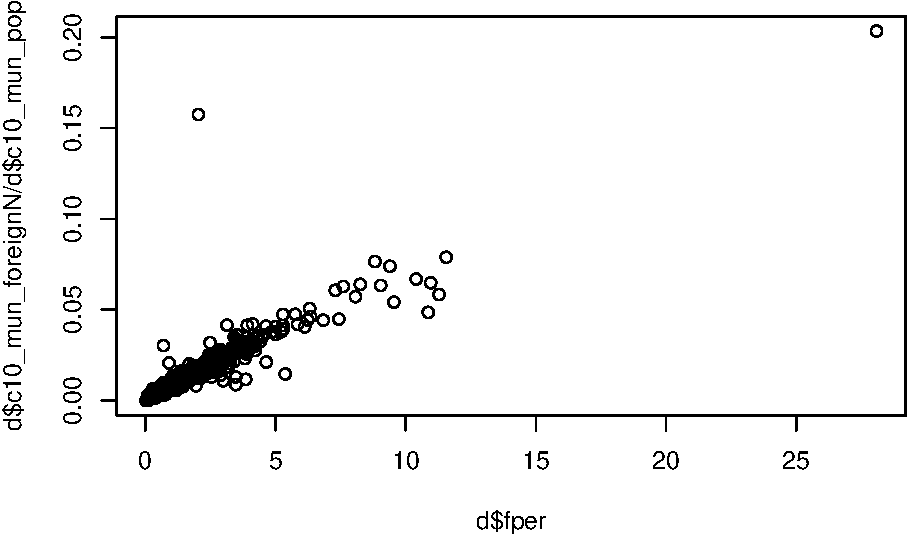
\includegraphics{visualization_2_matching_v5_files/figure-latex/unnamed-chunk-2-1.pdf}

\begin{Shaded}
\begin{Highlighting}[]
\KeywordTok{ggsave}\NormalTok{(}\KeywordTok{paste0}\NormalTok{(projdir,}\StringTok{"/out/matchbalanceplot_sifcct_v5.pdf"}\NormalTok{),p,}\DataTypeTok{width=}\DecValTok{8}\NormalTok{,}\DataTypeTok{height=}\DecValTok{5}\NormalTok{)}
\end{Highlighting}
\end{Shaded}

\hypertarget{plotting-geographic-distance-balance}{%
\section{Plotting Geographic Distance
Balance}\label{plotting-geographic-distance-balance}}

\hypertarget{prepare-japanese-map-data}{%
\subsection{Prepare Japanese Map Data}\label{prepare-japanese-map-data}}

\begin{Shaded}
\begin{Highlighting}[]
\CommentTok{## Referenced from https://uribo.hatenablog.com/entry/2017/12/08/144549}
\CommentTok{## All w/o Tokyo and Okinawa}
\NormalTok{alljp_no1347 <-}\StringTok{ }\KeywordTok{do.call}\NormalTok{(}\StringTok{"rbind"}\NormalTok{, }\KeywordTok{pblapply}\NormalTok{(}\KeywordTok{seq}\NormalTok{(}\DecValTok{1}\NormalTok{,}\DecValTok{47}\NormalTok{)[}\OperatorTok{-}\KeywordTok{c}\NormalTok{(}\DecValTok{13}\NormalTok{,}\DecValTok{47}\NormalTok{)], }
                                          \ControlFlowTok{function}\NormalTok{(k) }\KeywordTok{jpn_pref}\NormalTok{(}\DataTypeTok{pref_code =}\NormalTok{ k, }\DataTypeTok{district=}\OtherTok{FALSE}\NormalTok{)))}
\CommentTok{## Tokyo }
\NormalTok{tokyo13 <-}\StringTok{ }\KeywordTok{jpn_pref}\NormalTok{(}\DataTypeTok{pref_code =} \DecValTok{13}\NormalTok{, }\DataTypeTok{district =} \OtherTok{FALSE}\NormalTok{) }\OperatorTok\StringTok{ }
\StringTok{  }\KeywordTok{st_simplify}\NormalTok{(}\DataTypeTok{dTolerance =} \FloatTok{0.01}\NormalTok{)}
\end{Highlighting}
\end{Shaded}

\begin{verbatim}
## Warning in st_simplify.sfc(st_geometry(x), preserveTopology, dTolerance): st_simplify does not correctly simplify
## longitude/latitude data, dTolerance needs to be in decimal degrees
\end{verbatim}

\begin{Shaded}
\begin{Highlighting}[]
\CommentTok{## (Excluding Southern Islands) # Deprecated}
\CommentTok{# tokyo13 <- jpn_pref(pref_code = 13, district = TRUE) %>% }
\CommentTok{#   st_simplify(dTolerance = 0.01) %>% }
\CommentTok{#   mutate(city_code = as.numeric(city_code)) %>% }
\CommentTok{#   filter(city_code != 13421) %>% st_union() %>% }
\CommentTok{#   as.data.frame() %>% mutate(jis_code = "13", }
\CommentTok{#                              prefecture = "東京都") %>% magrittr::set_names(c("geometry", }
\CommentTok{#                                                                            "jis_code", "prefecture")) %>% st_as_sf()}
\CommentTok{## Okinawa }
\NormalTok{okinawa47 <-}\StringTok{ }\KeywordTok{jpn_pref}\NormalTok{(}\DataTypeTok{pref_code =} \DecValTok{47}\NormalTok{, }\DataTypeTok{district =} \OtherTok{FALSE}\NormalTok{)}
\NormalTok{okinawa47 <-}\StringTok{ }\NormalTok{okinawa47 }\OperatorTok\StringTok{ }\KeywordTok{st_set_crs}\NormalTok{(}\DataTypeTok{value =} \DecValTok{4326}\NormalTok{)}
\end{Highlighting}
\end{Shaded}

\hypertarget{prepare-respondents-data}{%
\subsection{Prepare Respondents Data}\label{prepare-respondents-data}}

\begin{Shaded}
\begin{Highlighting}[]
\CommentTok{# Sample N Respondents}
\NormalTok{N =}\StringTok{ }\DecValTok{200}
\KeywordTok{set.seed}\NormalTok{(}\DecValTok{3451}\NormalTok{)}
\NormalTok{dymap1 <-}\StringTok{ }\NormalTok{dym1[}\KeywordTok{which}\NormalTok{(dym1}\OperatorTok{$}\NormalTok{pair_id}\OperatorTok\KeywordTok{sample}\NormalTok{(dym1}\OperatorTok{$}\NormalTok{pair_id,N)),]}
\KeywordTok{set.seed}\NormalTok{(}\DecValTok{5412}\NormalTok{)}
\NormalTok{dymap2 <-}\StringTok{ }\NormalTok{dym2[}\KeywordTok{which}\NormalTok{(dym2}\OperatorTok{$}\NormalTok{pair_id}\OperatorTok\KeywordTok{sample}\NormalTok{(dym2}\OperatorTok{$}\NormalTok{pair_id,N)),]}
\KeywordTok{set.seed}\NormalTok{(}\DecValTok{5241}\NormalTok{)}
\NormalTok{dymap3 <-}\StringTok{ }\NormalTok{dym3[}\KeywordTok{which}\NormalTok{(dym3}\OperatorTok{$}\NormalTok{pair_id}\OperatorTok\KeywordTok{sample}\NormalTok{(dym3}\OperatorTok{$}\NormalTok{pair_id,N)),]}
\KeywordTok{set.seed}\NormalTok{(}\DecValTok{5441}\NormalTok{)}
\NormalTok{dymap4 <-}\StringTok{ }\NormalTok{dym4[}\KeywordTok{which}\NormalTok{(dym4}\OperatorTok{$}\NormalTok{pair_id}\OperatorTok\KeywordTok{sample}\NormalTok{(dym4}\OperatorTok{$}\NormalTok{pair_id,N)),]}
\KeywordTok{set.seed}\NormalTok{(}\DecValTok{5141}\NormalTok{)}
\NormalTok{dymap5 <-}\StringTok{ }\NormalTok{dym5[}\KeywordTok{which}\NormalTok{(dym5}\OperatorTok{$}\NormalTok{pair_id}\OperatorTok\KeywordTok{sample}\NormalTok{(dym5}\OperatorTok{$}\NormalTok{pair_id,N)),]}

\CommentTok{# Move Okinawa location to left-upper corner (not done for now) }
\CommentTok{# okinawa47$geometry <- okinawa47$geometry %>% magrittr::add(c(5.6, 17.5))}
\CommentTok{# dymap1$zip_lon[which(dymap1$zip_pref=="沖縄県")] <- dymap1$zip_lon[which(dymap1$zip_pref=="沖縄県")] + 5.6}
\CommentTok{# dymap1$zip_lat[which(dymap1$zip_pref=="沖縄県")] <- dymap1$zip_lat[which(dymap1$zip_pref=="沖縄県")] + 17.5}
\CommentTok{# dymap2$zip_lon[which(dymap2$zip_pref=="沖縄県")] <- dymap2$zip_lon[which(dymap2$zip_pref=="沖縄県")] + 5.6}
\CommentTok{# dymap2$zip_lat[which(dymap2$zip_pref=="沖縄県")] <- dymap2$zip_lat[which(dymap2$zip_pref=="沖縄県")] + 17.5}
\CommentTok{# dmmap1$zip_lon[which(dmmap1$zip_pref=="沖縄県")] <- dmmap1$zip_lon[which(dmmap1$zip_pref=="沖縄県")] + 5.6}
\CommentTok{# dmmap1$zip_lat[which(dmmap1$zip_pref=="沖縄県")] <- dmmap1$zip_lat[which(dmmap1$zip_pref=="沖縄県")] + 17.5}
\CommentTok{# dmmap2$zip_lon[which(dmmap2$zip_pref=="沖縄県")] <- dmmap2$zip_lon[which(dmmap2$zip_pref=="沖縄県")] + 5.6}
\CommentTok{# dmmap2$zip_lat[which(dmmap2$zip_pref=="沖縄県")] <- dmmap2$zip_lat[which(dmmap2$zip_pref=="沖縄県")] + 17.5}
\CommentTok{# demap1$zip_lon[which(demap1$zip_pref=="沖縄県")] <- demap1$zip_lon[which(demap1$zip_pref=="沖縄県")] + 5.6}
\CommentTok{# demap1$zip_lat[which(demap1$zip_pref=="沖縄県")] <- demap1$zip_lat[which(demap1$zip_pref=="沖縄県")] + 17.5}
\CommentTok{# demap2$zip_lon[which(demap2$zip_pref=="沖縄県")] <- demap2$zip_lon[which(demap2$zip_pref=="沖縄県")] + 5.6}
\CommentTok{# demap2$zip_lat[which(demap2$zip_pref=="沖縄県")] <- demap2$zip_lat[which(demap2$zip_pref=="沖縄県")] + 17.5}
\end{Highlighting}
\end{Shaded}

\hypertarget{plot}{%
\subsection{Plot}\label{plot}}

\begin{Shaded}
\begin{Highlighting}[]
\NormalTok{p1 <-}\StringTok{ }\KeywordTok{ggplot}\NormalTok{() }\OperatorTok{+}\StringTok{ }
\StringTok{  }\KeywordTok{geom_sf}\NormalTok{(}\DataTypeTok{data=}\NormalTok{alljp_no1347 }\OperatorTok\StringTok{ }\KeywordTok{st_simplify}\NormalTok{(}\DataTypeTok{dTolerance =} \FloatTok{0.01}\NormalTok{), }\DataTypeTok{size=}\FloatTok{0.3}\NormalTok{) }\OperatorTok{+}\StringTok{ }
\StringTok{  }\KeywordTok{geom_sf}\NormalTok{(}\DataTypeTok{data =}\NormalTok{ tokyo13, }\DataTypeTok{inherit.aes =} \OtherTok{TRUE}\NormalTok{, }\DataTypeTok{size=}\FloatTok{0.3}\NormalTok{) }\OperatorTok{+}\StringTok{ }
\StringTok{  }\KeywordTok{geom_sf}\NormalTok{(}\DataTypeTok{data =}\NormalTok{ okinawa47 }\OperatorTok\StringTok{ }\KeywordTok{st_simplify}\NormalTok{(}\DataTypeTok{dTolerance =} \FloatTok{0.01}\NormalTok{), }\DataTypeTok{inherit.aes =} \OtherTok{TRUE}\NormalTok{, }\DataTypeTok{size=}\FloatTok{0.3}\NormalTok{) }\OperatorTok{+}\StringTok{   }
\StringTok{  }\CommentTok{# geom_segment(aes(x = round(st_bbox(alljp_no1347)[1], 0), xend = 132.5, y = 40, yend = 40)) + }
\StringTok{  }\CommentTok{# geom_segment(aes(x = 132.5, xend = 138, y = 40, yend = 42)) + }
\StringTok{  }\CommentTok{# geom_segment(aes(x = 138, xend = 138, y = 42, yend = round(st_bbox(alljp_no1347)[4],0))) + }
\StringTok{  }\KeywordTok{geom_point}\NormalTok{(}\DataTypeTok{data =}\NormalTok{ dymap1, }\KeywordTok{aes}\NormalTok{(}\DataTypeTok{x=}\NormalTok{zip_lon,}\DataTypeTok{y=}\NormalTok{zip_lat, }\DataTypeTok{color=}\KeywordTok{as.factor}\NormalTok{(}\DecValTok{1}\OperatorTok{-}\NormalTok{female)), }\DataTypeTok{alpha=}\FloatTok{0.5}\NormalTok{, }\DataTypeTok{size=}\FloatTok{0.4}\NormalTok{) }\OperatorTok{+}\StringTok{ }
\StringTok{  }\KeywordTok{geom_path}\NormalTok{(}\DataTypeTok{data =}\NormalTok{ dymap1, }\KeywordTok{aes}\NormalTok{(}\DataTypeTok{x=}\NormalTok{zip_lon,}\DataTypeTok{y=}\NormalTok{zip_lat, }\DataTypeTok{group=}\NormalTok{pair_id, }\DataTypeTok{color=}\KeywordTok{as.factor}\NormalTok{(}\DecValTok{1}\OperatorTok{-}\NormalTok{female)), }\DataTypeTok{alpha=}\FloatTok{0.65}\NormalTok{, }\DataTypeTok{size=}\FloatTok{0.3}\NormalTok{) }\OperatorTok{+}\StringTok{ }
\StringTok{  }\KeywordTok{scale_color_manual}\NormalTok{(}\DataTypeTok{name=}\StringTok{"Gender"}\NormalTok{, }\DataTypeTok{values=}\KeywordTok{c}\NormalTok{(}\StringTok{"darkred"}\NormalTok{,}\StringTok{"navyblue"}\NormalTok{)) }\OperatorTok{+}\StringTok{ }
\StringTok{  }\KeywordTok{coord_sf}\NormalTok{(}\DataTypeTok{xlim=}\KeywordTok{c}\NormalTok{(}\FloatTok{124.5}\NormalTok{,}\FloatTok{148.5}\NormalTok{)) }\OperatorTok{+}\StringTok{ }
\StringTok{  }\CommentTok{#coord_sf(xlim=c(128,148.5),ylim=c(27,46)) + }
\StringTok{  }\KeywordTok{labs}\NormalTok{(}\DataTypeTok{x=}\KeywordTok{paste0}\NormalTok{(}\KeywordTok{table}\NormalTok{(dym1[dym1}\OperatorTok{$}\NormalTok{female}\OperatorTok{==}\DecValTok{1}\NormalTok{,]}\OperatorTok{$}\NormalTok{treated)[}\DecValTok{1}\NormalTok{],}\StringTok{"/"}\NormalTok{,}\KeywordTok{table}\NormalTok{(dy[dy}\OperatorTok{$}\NormalTok{female}\OperatorTok{==}\DecValTok{1}\NormalTok{,]}\OperatorTok{$}\NormalTok{edu2)[}\DecValTok{2}\NormalTok{],}\StringTok{" Female and "}\NormalTok{,}
                \KeywordTok{table}\NormalTok{(dym1[dym1}\OperatorTok{$}\NormalTok{female}\OperatorTok{==}\DecValTok{0}\NormalTok{,]}\OperatorTok{$}\NormalTok{treated)[}\DecValTok{1}\NormalTok{],}\StringTok{"/"}\NormalTok{,}\KeywordTok{table}\NormalTok{(dy[dy}\OperatorTok{$}\NormalTok{female}\OperatorTok{==}\DecValTok{0}\NormalTok{,]}\OperatorTok{$}\NormalTok{edu2)[}\DecValTok{1}\NormalTok{],}
                \StringTok{" Male Matched Pairs Found"}\NormalTok{),}
       \DataTypeTok{y=}\OtherTok{NULL}\NormalTok{,}\DataTypeTok{title=}\StringTok{"No Distance Adjustment"}\NormalTok{) }\OperatorTok{+}\StringTok{ }\KeywordTok{theme_light}\NormalTok{() }\OperatorTok{+}\StringTok{ }
\StringTok{  }\KeywordTok{theme}\NormalTok{(}\DataTypeTok{plot.title=}\KeywordTok{element_text}\NormalTok{(}\DataTypeTok{hjust=}\FloatTok{0.5}\NormalTok{),}
        \DataTypeTok{panel.background =} \KeywordTok{element_rect}\NormalTok{(}\DataTypeTok{color=}\StringTok{"black"}\NormalTok{,}\DataTypeTok{fill=}\StringTok{"white"}\NormalTok{),}
        \DataTypeTok{axis.ticks =} \KeywordTok{element_blank}\NormalTok{(),}
        \DataTypeTok{axis.text =} \KeywordTok{element_blank}\NormalTok{(),}
        \DataTypeTok{line =} \KeywordTok{element_blank}\NormalTok{(), }
        \DataTypeTok{axis.title.x =} \KeywordTok{element_text}\NormalTok{(}\DataTypeTok{size=}\DecValTok{10}\NormalTok{),}
        \DataTypeTok{legend.position =} \StringTok{"none"}\NormalTok{)}
\end{Highlighting}
\end{Shaded}

\begin{verbatim}
## Warning in st_simplify.sfc(st_geometry(x), preserveTopology, dTolerance): st_simplify does not correctly simplify
## longitude/latitude data, dTolerance needs to be in decimal degrees

## Warning in st_simplify.sfc(st_geometry(x), preserveTopology, dTolerance): st_simplify does not correctly simplify
## longitude/latitude data, dTolerance needs to be in decimal degrees
\end{verbatim}

\begin{Shaded}
\begin{Highlighting}[]
\NormalTok{p1}
\end{Highlighting}
\end{Shaded}

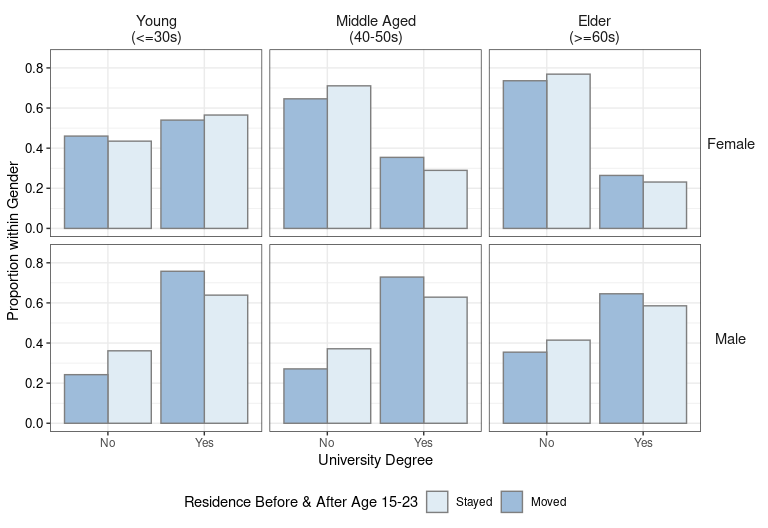
\includegraphics{visualization_2_matching_v5_files/figure-latex/unnamed-chunk-6-1.pdf}

\begin{Shaded}
\begin{Highlighting}[]
\NormalTok{p2 <-}\StringTok{ }\KeywordTok{ggplot}\NormalTok{() }\OperatorTok{+}\StringTok{ }
\StringTok{  }\KeywordTok{geom_sf}\NormalTok{(}\DataTypeTok{data=}\NormalTok{alljp_no1347 }\OperatorTok\StringTok{ }\KeywordTok{st_simplify}\NormalTok{(}\DataTypeTok{dTolerance =} \FloatTok{0.01}\NormalTok{), }\DataTypeTok{size=}\FloatTok{0.3}\NormalTok{) }\OperatorTok{+}\StringTok{ }
\StringTok{  }\KeywordTok{geom_sf}\NormalTok{(}\DataTypeTok{data =}\NormalTok{ tokyo13, }\DataTypeTok{inherit.aes =} \OtherTok{TRUE}\NormalTok{, }\DataTypeTok{size=}\FloatTok{0.3}\NormalTok{) }\OperatorTok{+}\StringTok{ }
\StringTok{  }\KeywordTok{geom_sf}\NormalTok{(}\DataTypeTok{data =}\NormalTok{ okinawa47 }\OperatorTok\StringTok{ }\KeywordTok{st_simplify}\NormalTok{(}\DataTypeTok{dTolerance =} \FloatTok{0.01}\NormalTok{), }\DataTypeTok{inherit.aes =} \OtherTok{TRUE}\NormalTok{, }\DataTypeTok{size=}\FloatTok{0.3}\NormalTok{) }\OperatorTok{+}\StringTok{   }
\StringTok{  }\CommentTok{# geom_segment(aes(x = round(st_bbox(alljp_no1347)[1], 0), xend = 132.5, y = 40, yend = 40)) + }
\StringTok{  }\CommentTok{# geom_segment(aes(x = 132.5, xend = 138, y = 40, yend = 42)) + }
\StringTok{  }\CommentTok{# geom_segment(aes(x = 138, xend = 138, y = 42, yend = round(st_bbox(alljp_no1347)[4],0))) + }
\StringTok{  }\KeywordTok{geom_point}\NormalTok{(}\DataTypeTok{data =}\NormalTok{ dymap2, }\KeywordTok{aes}\NormalTok{(}\DataTypeTok{x=}\NormalTok{zip_lon,}\DataTypeTok{y=}\NormalTok{zip_lat, }\DataTypeTok{color=}\KeywordTok{as.factor}\NormalTok{(}\DecValTok{1}\OperatorTok{-}\NormalTok{female)), }\DataTypeTok{alpha=}\FloatTok{0.5}\NormalTok{, }\DataTypeTok{size=}\FloatTok{0.4}\NormalTok{) }\OperatorTok{+}\StringTok{ }
\StringTok{  }\KeywordTok{geom_path}\NormalTok{(}\DataTypeTok{data =}\NormalTok{ dymap2, }\KeywordTok{aes}\NormalTok{(}\DataTypeTok{x=}\NormalTok{zip_lon,}\DataTypeTok{y=}\NormalTok{zip_lat, }\DataTypeTok{group=}\NormalTok{pair_id, }\DataTypeTok{color=}\KeywordTok{as.factor}\NormalTok{(}\DecValTok{1}\OperatorTok{-}\NormalTok{female)), }\DataTypeTok{alpha=}\FloatTok{0.8}\NormalTok{, }\DataTypeTok{size=}\FloatTok{0.3}\NormalTok{) }\OperatorTok{+}\StringTok{ }
\StringTok{  }\KeywordTok{scale_color_manual}\NormalTok{(}\DataTypeTok{name=}\StringTok{"Gender"}\NormalTok{, }\DataTypeTok{values=}\KeywordTok{c}\NormalTok{(}\StringTok{"darkred"}\NormalTok{,}\StringTok{"navyblue"}\NormalTok{)) }\OperatorTok{+}\StringTok{ }
\StringTok{  }\KeywordTok{coord_sf}\NormalTok{(}\DataTypeTok{xlim=}\KeywordTok{c}\NormalTok{(}\FloatTok{124.5}\NormalTok{,}\FloatTok{148.5}\NormalTok{)) }\OperatorTok{+}\StringTok{ }
\StringTok{  }\CommentTok{#coord_sf(xlim=c(128,148.5),ylim=c(27,46)) + }
\StringTok{  }\KeywordTok{labs}\NormalTok{(}\DataTypeTok{x=}\KeywordTok{paste0}\NormalTok{(}\KeywordTok{table}\NormalTok{(dym2[dym2}\OperatorTok{$}\NormalTok{female}\OperatorTok{==}\DecValTok{1}\NormalTok{,]}\OperatorTok{$}\NormalTok{treated)[}\DecValTok{1}\NormalTok{],}\StringTok{"/"}\NormalTok{,}\KeywordTok{table}\NormalTok{(dy[dy}\OperatorTok{$}\NormalTok{female}\OperatorTok{==}\DecValTok{1}\NormalTok{,]}\OperatorTok{$}\NormalTok{edu2)[}\DecValTok{2}\NormalTok{],}\StringTok{" Female and "}\NormalTok{,}
                \KeywordTok{table}\NormalTok{(dym2[dym2}\OperatorTok{$}\NormalTok{female}\OperatorTok{==}\DecValTok{0}\NormalTok{,]}\OperatorTok{$}\NormalTok{treated)[}\DecValTok{1}\NormalTok{],}\StringTok{"/"}\NormalTok{,}\KeywordTok{table}\NormalTok{(dy[dy}\OperatorTok{$}\NormalTok{female}\OperatorTok{==}\DecValTok{0}\NormalTok{,]}\OperatorTok{$}\NormalTok{edu2)[}\DecValTok{1}\NormalTok{],}
                \StringTok{" Male Matched Pairs Found"}\NormalTok{),}
       \DataTypeTok{y=}\OtherTok{NULL}\NormalTok{,}\DataTypeTok{title=}\KeywordTok{bquote}\NormalTok{(}\StringTok{"Distance Adjusted ("}\OperatorTok{~}\NormalTok{lambda}\OperatorTok{~}\StringTok{" = 50km)"}\NormalTok{)) }\OperatorTok{+}\StringTok{ }\KeywordTok{theme_light}\NormalTok{() }\OperatorTok{+}\StringTok{ }
\StringTok{  }\KeywordTok{theme}\NormalTok{(}\DataTypeTok{plot.title=}\KeywordTok{element_text}\NormalTok{(}\DataTypeTok{hjust=}\FloatTok{0.5}\NormalTok{),}
        \DataTypeTok{panel.background =} \KeywordTok{element_rect}\NormalTok{(}\DataTypeTok{color=}\StringTok{"black"}\NormalTok{,}\DataTypeTok{fill=}\StringTok{"white"}\NormalTok{),}
        \DataTypeTok{axis.ticks =} \KeywordTok{element_blank}\NormalTok{(),}
        \DataTypeTok{axis.text =} \KeywordTok{element_blank}\NormalTok{(),}
        \DataTypeTok{line =} \KeywordTok{element_blank}\NormalTok{(), }
        \DataTypeTok{axis.title.x =} \KeywordTok{element_text}\NormalTok{(}\DataTypeTok{size=}\DecValTok{10}\NormalTok{),}
        \DataTypeTok{legend.position =} \StringTok{"none"}\NormalTok{)}
\end{Highlighting}
\end{Shaded}

\begin{verbatim}
## Warning in st_simplify.sfc(st_geometry(x), preserveTopology, dTolerance): st_simplify does not correctly simplify
## longitude/latitude data, dTolerance needs to be in decimal degrees

## Warning in st_simplify.sfc(st_geometry(x), preserveTopology, dTolerance): st_simplify does not correctly simplify
## longitude/latitude data, dTolerance needs to be in decimal degrees
\end{verbatim}

\begin{Shaded}
\begin{Highlighting}[]
\NormalTok{p2}
\end{Highlighting}
\end{Shaded}

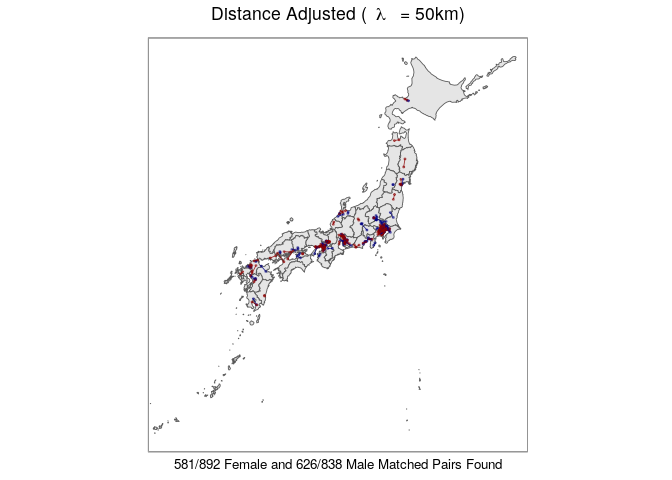
\includegraphics{visualization_2_matching_v5_files/figure-latex/unnamed-chunk-6-2.pdf}

\begin{Shaded}
\begin{Highlighting}[]
\NormalTok{p3 <-}\StringTok{ }\KeywordTok{ggplot}\NormalTok{() }\OperatorTok{+}\StringTok{ }
\StringTok{  }\KeywordTok{geom_sf}\NormalTok{(}\DataTypeTok{data=}\NormalTok{alljp_no1347 }\OperatorTok\StringTok{ }\KeywordTok{st_simplify}\NormalTok{(}\DataTypeTok{dTolerance =} \FloatTok{0.01}\NormalTok{), }\DataTypeTok{size=}\FloatTok{0.3}\NormalTok{) }\OperatorTok{+}\StringTok{ }
\StringTok{  }\KeywordTok{geom_sf}\NormalTok{(}\DataTypeTok{data =}\NormalTok{ tokyo13, }\DataTypeTok{inherit.aes =} \OtherTok{TRUE}\NormalTok{, }\DataTypeTok{size=}\FloatTok{0.3}\NormalTok{) }\OperatorTok{+}\StringTok{ }
\StringTok{  }\KeywordTok{geom_sf}\NormalTok{(}\DataTypeTok{data =}\NormalTok{ okinawa47 }\OperatorTok\StringTok{ }\KeywordTok{st_simplify}\NormalTok{(}\DataTypeTok{dTolerance =} \FloatTok{0.01}\NormalTok{), }\DataTypeTok{inherit.aes =} \OtherTok{TRUE}\NormalTok{, }\DataTypeTok{size=}\FloatTok{0.3}\NormalTok{) }\OperatorTok{+}\StringTok{   }
\StringTok{  }\CommentTok{# geom_segment(aes(x = round(st_bbox(alljp_no1347)[1], 0), xend = 132.5, y = 40, yend = 40)) + }
\StringTok{  }\CommentTok{# geom_segment(aes(x = 132.5, xend = 138, y = 40, yend = 42)) + }
\StringTok{  }\CommentTok{# geom_segment(aes(x = 138, xend = 138, y = 42, yend = round(st_bbox(alljp_no1347)[4],0))) + }
\StringTok{  }\KeywordTok{geom_point}\NormalTok{(}\DataTypeTok{data =}\NormalTok{ dymap3, }\KeywordTok{aes}\NormalTok{(}\DataTypeTok{x=}\NormalTok{zip_lon,}\DataTypeTok{y=}\NormalTok{zip_lat, }\DataTypeTok{color=}\KeywordTok{as.factor}\NormalTok{(}\DecValTok{1}\OperatorTok{-}\NormalTok{female)), }\DataTypeTok{alpha=}\FloatTok{0.5}\NormalTok{, }\DataTypeTok{size=}\FloatTok{0.4}\NormalTok{) }\OperatorTok{+}\StringTok{ }
\StringTok{  }\KeywordTok{geom_path}\NormalTok{(}\DataTypeTok{data =}\NormalTok{ dymap3, }\KeywordTok{aes}\NormalTok{(}\DataTypeTok{x=}\NormalTok{zip_lon,}\DataTypeTok{y=}\NormalTok{zip_lat, }\DataTypeTok{group=}\NormalTok{pair_id, }\DataTypeTok{color=}\KeywordTok{as.factor}\NormalTok{(}\DecValTok{1}\OperatorTok{-}\NormalTok{female)), }\DataTypeTok{alpha=}\FloatTok{0.8}\NormalTok{, }\DataTypeTok{size=}\FloatTok{0.3}\NormalTok{) }\OperatorTok{+}\StringTok{ }
\StringTok{  }\KeywordTok{scale_color_manual}\NormalTok{(}\DataTypeTok{name=}\StringTok{"Gender"}\NormalTok{, }\DataTypeTok{values=}\KeywordTok{c}\NormalTok{(}\StringTok{"darkred"}\NormalTok{,}\StringTok{"navyblue"}\NormalTok{)) }\OperatorTok{+}\StringTok{ }
\StringTok{  }\KeywordTok{coord_sf}\NormalTok{(}\DataTypeTok{xlim=}\KeywordTok{c}\NormalTok{(}\FloatTok{124.5}\NormalTok{,}\FloatTok{148.5}\NormalTok{)) }\OperatorTok{+}\StringTok{ }
\StringTok{  }\CommentTok{#coord_sf(xlim=c(128,148.5),ylim=c(27,46)) + }
\StringTok{  }\KeywordTok{labs}\NormalTok{(}\DataTypeTok{x=}\KeywordTok{paste0}\NormalTok{(}\KeywordTok{table}\NormalTok{(dym3[dym3}\OperatorTok{$}\NormalTok{female}\OperatorTok{==}\DecValTok{1}\NormalTok{,]}\OperatorTok{$}\NormalTok{treated)[}\DecValTok{1}\NormalTok{],}\StringTok{"/"}\NormalTok{,}\KeywordTok{table}\NormalTok{(dy[dy}\OperatorTok{$}\NormalTok{female}\OperatorTok{==}\DecValTok{1}\NormalTok{,]}\OperatorTok{$}\NormalTok{edu2)[}\DecValTok{2}\NormalTok{],}\StringTok{" Female and "}\NormalTok{,}
                \KeywordTok{table}\NormalTok{(dym3[dym3}\OperatorTok{$}\NormalTok{female}\OperatorTok{==}\DecValTok{0}\NormalTok{,]}\OperatorTok{$}\NormalTok{treated)[}\DecValTok{1}\NormalTok{],}\StringTok{"/"}\NormalTok{,}\KeywordTok{table}\NormalTok{(dy[dy}\OperatorTok{$}\NormalTok{female}\OperatorTok{==}\DecValTok{0}\NormalTok{,]}\OperatorTok{$}\NormalTok{edu2)[}\DecValTok{1}\NormalTok{],}
                \StringTok{" Male Matched Pairs Found"}\NormalTok{),}
       \DataTypeTok{y=}\OtherTok{NULL}\NormalTok{,}\DataTypeTok{title=}\KeywordTok{bquote}\NormalTok{(}\StringTok{"Distance Adjusted ("}\OperatorTok{~}\NormalTok{lambda}\OperatorTok{~}\StringTok{" = 100km)"}\NormalTok{)) }\OperatorTok{+}\StringTok{ }\KeywordTok{theme_light}\NormalTok{() }\OperatorTok{+}\StringTok{ }
\StringTok{  }\KeywordTok{theme}\NormalTok{(}\DataTypeTok{plot.title=}\KeywordTok{element_text}\NormalTok{(}\DataTypeTok{hjust=}\FloatTok{0.5}\NormalTok{),}
        \DataTypeTok{panel.background =} \KeywordTok{element_rect}\NormalTok{(}\DataTypeTok{color=}\StringTok{"black"}\NormalTok{,}\DataTypeTok{fill=}\StringTok{"white"}\NormalTok{),}
        \DataTypeTok{axis.ticks =} \KeywordTok{element_blank}\NormalTok{(),}
        \DataTypeTok{axis.text =} \KeywordTok{element_blank}\NormalTok{(),}
        \DataTypeTok{line =} \KeywordTok{element_blank}\NormalTok{(), }
        \DataTypeTok{axis.title.x =} \KeywordTok{element_text}\NormalTok{(}\DataTypeTok{size=}\DecValTok{10}\NormalTok{),}
        \DataTypeTok{legend.position =} \StringTok{"none"}\NormalTok{)}
\end{Highlighting}
\end{Shaded}

\begin{verbatim}
## Warning in st_simplify.sfc(st_geometry(x), preserveTopology, dTolerance): st_simplify does not correctly simplify
## longitude/latitude data, dTolerance needs to be in decimal degrees

## Warning in st_simplify.sfc(st_geometry(x), preserveTopology, dTolerance): st_simplify does not correctly simplify
## longitude/latitude data, dTolerance needs to be in decimal degrees
\end{verbatim}

\begin{Shaded}
\begin{Highlighting}[]
\NormalTok{p3}
\end{Highlighting}
\end{Shaded}

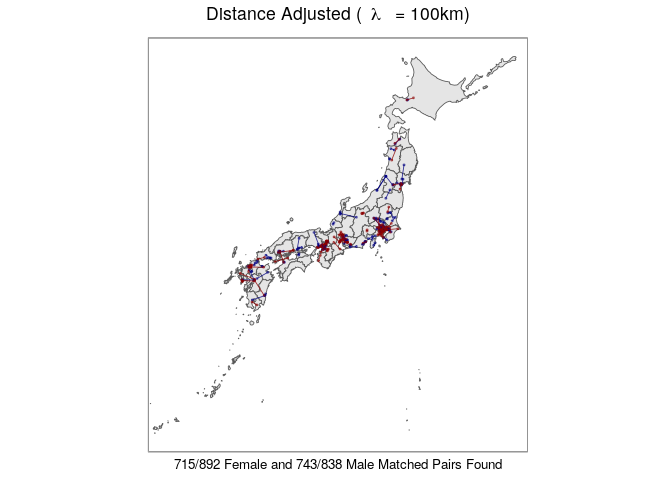
\includegraphics{visualization_2_matching_v5_files/figure-latex/unnamed-chunk-6-3.pdf}

\begin{Shaded}
\begin{Highlighting}[]
\NormalTok{p4 <-}\StringTok{ }\KeywordTok{ggplot}\NormalTok{() }\OperatorTok{+}\StringTok{ }
\StringTok{  }\KeywordTok{geom_sf}\NormalTok{(}\DataTypeTok{data=}\NormalTok{alljp_no1347 }\OperatorTok\StringTok{ }\KeywordTok{st_simplify}\NormalTok{(}\DataTypeTok{dTolerance =} \FloatTok{0.01}\NormalTok{), }\DataTypeTok{size=}\FloatTok{0.3}\NormalTok{) }\OperatorTok{+}\StringTok{ }
\StringTok{  }\KeywordTok{geom_sf}\NormalTok{(}\DataTypeTok{data =}\NormalTok{ tokyo13, }\DataTypeTok{inherit.aes =} \OtherTok{TRUE}\NormalTok{, }\DataTypeTok{size=}\FloatTok{0.3}\NormalTok{) }\OperatorTok{+}\StringTok{ }
\StringTok{  }\KeywordTok{geom_sf}\NormalTok{(}\DataTypeTok{data =}\NormalTok{ okinawa47 }\OperatorTok\StringTok{ }\KeywordTok{st_simplify}\NormalTok{(}\DataTypeTok{dTolerance =} \FloatTok{0.01}\NormalTok{), }\DataTypeTok{inherit.aes =} \OtherTok{TRUE}\NormalTok{, }\DataTypeTok{size=}\FloatTok{0.3}\NormalTok{) }\OperatorTok{+}\StringTok{   }
\StringTok{  }\CommentTok{# geom_segment(aes(x = round(st_bbox(alljp_no1347)[1], 0), xend = 132.5, y = 40, yend = 40)) + }
\StringTok{  }\CommentTok{# geom_segment(aes(x = 132.5, xend = 138, y = 40, yend = 42)) + }
\StringTok{  }\CommentTok{# geom_segment(aes(x = 138, xend = 138, y = 42, yend = round(st_bbox(alljp_no1347)[4],0))) + }
\StringTok{  }\KeywordTok{geom_point}\NormalTok{(}\DataTypeTok{data =}\NormalTok{ dymap4, }\KeywordTok{aes}\NormalTok{(}\DataTypeTok{x=}\NormalTok{zip_lon,}\DataTypeTok{y=}\NormalTok{zip_lat, }\DataTypeTok{color=}\KeywordTok{as.factor}\NormalTok{(}\DecValTok{1}\OperatorTok{-}\NormalTok{female)), }\DataTypeTok{alpha=}\FloatTok{0.5}\NormalTok{, }\DataTypeTok{size=}\FloatTok{0.4}\NormalTok{) }\OperatorTok{+}\StringTok{ }
\StringTok{  }\KeywordTok{geom_path}\NormalTok{(}\DataTypeTok{data =}\NormalTok{ dymap4, }\KeywordTok{aes}\NormalTok{(}\DataTypeTok{x=}\NormalTok{zip_lon,}\DataTypeTok{y=}\NormalTok{zip_lat, }\DataTypeTok{group=}\NormalTok{pair_id, }\DataTypeTok{color=}\KeywordTok{as.factor}\NormalTok{(}\DecValTok{1}\OperatorTok{-}\NormalTok{female)), }\DataTypeTok{alpha=}\FloatTok{0.8}\NormalTok{, }\DataTypeTok{size=}\FloatTok{0.3}\NormalTok{) }\OperatorTok{+}\StringTok{ }
\StringTok{  }\KeywordTok{scale_color_manual}\NormalTok{(}\DataTypeTok{name=}\StringTok{"Gender"}\NormalTok{, }\DataTypeTok{values=}\KeywordTok{c}\NormalTok{(}\StringTok{"darkred"}\NormalTok{,}\StringTok{"navyblue"}\NormalTok{)) }\OperatorTok{+}\StringTok{ }
\StringTok{  }\KeywordTok{coord_sf}\NormalTok{(}\DataTypeTok{xlim=}\KeywordTok{c}\NormalTok{(}\FloatTok{124.5}\NormalTok{,}\FloatTok{148.5}\NormalTok{)) }\OperatorTok{+}\StringTok{ }
\StringTok{  }\CommentTok{#coord_sf(xlim=c(128,148.5),ylim=c(27,46)) + }
\StringTok{  }\KeywordTok{labs}\NormalTok{(}\DataTypeTok{x=}\KeywordTok{paste0}\NormalTok{(}\KeywordTok{table}\NormalTok{(dym4[dym4}\OperatorTok{$}\NormalTok{female}\OperatorTok{==}\DecValTok{1}\NormalTok{,]}\OperatorTok{$}\NormalTok{treated)[}\DecValTok{1}\NormalTok{],}\StringTok{"/"}\NormalTok{,}\KeywordTok{table}\NormalTok{(dy[dy}\OperatorTok{$}\NormalTok{female}\OperatorTok{==}\DecValTok{1}\NormalTok{,]}\OperatorTok{$}\NormalTok{edu2)[}\DecValTok{2}\NormalTok{],}\StringTok{" Female and "}\NormalTok{,}
                \KeywordTok{table}\NormalTok{(dym4[dym4}\OperatorTok{$}\NormalTok{female}\OperatorTok{==}\DecValTok{0}\NormalTok{,]}\OperatorTok{$}\NormalTok{treated)[}\DecValTok{1}\NormalTok{],}\StringTok{"/"}\NormalTok{,}\KeywordTok{table}\NormalTok{(dy[dy}\OperatorTok{$}\NormalTok{female}\OperatorTok{==}\DecValTok{0}\NormalTok{,]}\OperatorTok{$}\NormalTok{edu2)[}\DecValTok{1}\NormalTok{],}
                \StringTok{" Male Matched Pairs Found"}\NormalTok{),}
       \DataTypeTok{y=}\OtherTok{NULL}\NormalTok{,}\DataTypeTok{title=}\KeywordTok{bquote}\NormalTok{(}\StringTok{"Distance Adjusted ("}\OperatorTok{~}\NormalTok{lambda}\OperatorTok{~}\StringTok{" = 200km)"}\NormalTok{)) }\OperatorTok{+}\StringTok{ }\KeywordTok{theme_light}\NormalTok{() }\OperatorTok{+}\StringTok{ }
\StringTok{  }\KeywordTok{theme}\NormalTok{(}\DataTypeTok{plot.title=}\KeywordTok{element_text}\NormalTok{(}\DataTypeTok{hjust=}\FloatTok{0.5}\NormalTok{),}
        \DataTypeTok{panel.background =} \KeywordTok{element_rect}\NormalTok{(}\DataTypeTok{color=}\StringTok{"black"}\NormalTok{,}\DataTypeTok{fill=}\StringTok{"white"}\NormalTok{),}
        \DataTypeTok{axis.ticks =} \KeywordTok{element_blank}\NormalTok{(),}
        \DataTypeTok{axis.text =} \KeywordTok{element_blank}\NormalTok{(),}
        \DataTypeTok{line =} \KeywordTok{element_blank}\NormalTok{(), }
        \DataTypeTok{axis.title.x =} \KeywordTok{element_text}\NormalTok{(}\DataTypeTok{size=}\DecValTok{10}\NormalTok{),}
        \DataTypeTok{legend.position =} \StringTok{"none"}\NormalTok{)}
\end{Highlighting}
\end{Shaded}

\begin{verbatim}
## Warning in st_simplify.sfc(st_geometry(x), preserveTopology, dTolerance): st_simplify does not correctly simplify
## longitude/latitude data, dTolerance needs to be in decimal degrees

## Warning in st_simplify.sfc(st_geometry(x), preserveTopology, dTolerance): st_simplify does not correctly simplify
## longitude/latitude data, dTolerance needs to be in decimal degrees
\end{verbatim}

\begin{Shaded}
\begin{Highlighting}[]
\NormalTok{p4}
\end{Highlighting}
\end{Shaded}

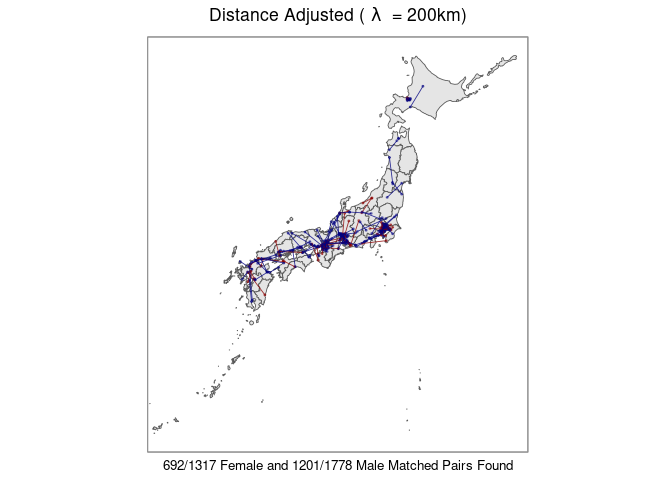
\includegraphics{visualization_2_matching_v5_files/figure-latex/unnamed-chunk-6-4.pdf}

\begin{Shaded}
\begin{Highlighting}[]
\NormalTok{p5 <-}\StringTok{ }\KeywordTok{ggplot}\NormalTok{() }\OperatorTok{+}\StringTok{ }
\StringTok{  }\KeywordTok{geom_sf}\NormalTok{(}\DataTypeTok{data=}\NormalTok{alljp_no1347 }\OperatorTok\StringTok{ }\KeywordTok{st_simplify}\NormalTok{(}\DataTypeTok{dTolerance =} \FloatTok{0.01}\NormalTok{), }\DataTypeTok{size=}\FloatTok{0.3}\NormalTok{) }\OperatorTok{+}\StringTok{ }
\StringTok{  }\KeywordTok{geom_sf}\NormalTok{(}\DataTypeTok{data =}\NormalTok{ tokyo13, }\DataTypeTok{inherit.aes =} \OtherTok{TRUE}\NormalTok{, }\DataTypeTok{size=}\FloatTok{0.3}\NormalTok{) }\OperatorTok{+}\StringTok{ }
\StringTok{  }\KeywordTok{geom_sf}\NormalTok{(}\DataTypeTok{data =}\NormalTok{ okinawa47 }\OperatorTok\StringTok{ }\KeywordTok{st_simplify}\NormalTok{(}\DataTypeTok{dTolerance =} \FloatTok{0.01}\NormalTok{), }\DataTypeTok{inherit.aes =} \OtherTok{TRUE}\NormalTok{, }\DataTypeTok{size=}\FloatTok{0.3}\NormalTok{) }\OperatorTok{+}\StringTok{   }
\StringTok{  }\CommentTok{# geom_segment(aes(x = round(st_bbox(alljp_no1347)[1], 0), xend = 132.5, y = 40, yend = 40)) + }
\StringTok{  }\CommentTok{# geom_segment(aes(x = 132.5, xend = 138, y = 40, yend = 42)) + }
\StringTok{  }\CommentTok{# geom_segment(aes(x = 138, xend = 138, y = 42, yend = round(st_bbox(alljp_no1347)[4],0))) + }
\StringTok{  }\KeywordTok{geom_point}\NormalTok{(}\DataTypeTok{data =}\NormalTok{ dymap5, }\KeywordTok{aes}\NormalTok{(}\DataTypeTok{x=}\NormalTok{zip_lon,}\DataTypeTok{y=}\NormalTok{zip_lat, }\DataTypeTok{color=}\KeywordTok{as.factor}\NormalTok{(}\DecValTok{1}\OperatorTok{-}\NormalTok{female)), }\DataTypeTok{alpha=}\FloatTok{0.5}\NormalTok{, }\DataTypeTok{size=}\FloatTok{0.4}\NormalTok{) }\OperatorTok{+}\StringTok{ }
\StringTok{  }\KeywordTok{geom_path}\NormalTok{(}\DataTypeTok{data =}\NormalTok{ dymap5, }\KeywordTok{aes}\NormalTok{(}\DataTypeTok{x=}\NormalTok{zip_lon,}\DataTypeTok{y=}\NormalTok{zip_lat, }\DataTypeTok{group=}\NormalTok{pair_id, }\DataTypeTok{color=}\KeywordTok{as.factor}\NormalTok{(}\DecValTok{1}\OperatorTok{-}\NormalTok{female)), }\DataTypeTok{alpha=}\FloatTok{0.8}\NormalTok{, }\DataTypeTok{size=}\FloatTok{0.3}\NormalTok{) }\OperatorTok{+}\StringTok{ }
\StringTok{  }\KeywordTok{scale_color_manual}\NormalTok{(}\DataTypeTok{name=}\StringTok{"Gender"}\NormalTok{, }\DataTypeTok{values=}\KeywordTok{c}\NormalTok{(}\StringTok{"darkred"}\NormalTok{,}\StringTok{"navyblue"}\NormalTok{)) }\OperatorTok{+}\StringTok{ }
\StringTok{  }\KeywordTok{coord_sf}\NormalTok{(}\DataTypeTok{xlim=}\KeywordTok{c}\NormalTok{(}\FloatTok{124.5}\NormalTok{,}\FloatTok{148.5}\NormalTok{)) }\OperatorTok{+}\StringTok{ }
\StringTok{  }\CommentTok{#coord_sf(xlim=c(128,148.5),ylim=c(27,46)) + }
\StringTok{  }\KeywordTok{labs}\NormalTok{(}\DataTypeTok{x=}\KeywordTok{paste0}\NormalTok{(}\KeywordTok{table}\NormalTok{(dym5[dym5}\OperatorTok{$}\NormalTok{female}\OperatorTok{==}\DecValTok{1}\NormalTok{,]}\OperatorTok{$}\NormalTok{treated)[}\DecValTok{1}\NormalTok{],}\StringTok{"/"}\NormalTok{,}\KeywordTok{table}\NormalTok{(dy[dy}\OperatorTok{$}\NormalTok{female}\OperatorTok{==}\DecValTok{1}\NormalTok{,]}\OperatorTok{$}\NormalTok{edu2)[}\DecValTok{2}\NormalTok{],}\StringTok{" Female and "}\NormalTok{,}
                \KeywordTok{table}\NormalTok{(dym5[dym5}\OperatorTok{$}\NormalTok{female}\OperatorTok{==}\DecValTok{0}\NormalTok{,]}\OperatorTok{$}\NormalTok{treated)[}\DecValTok{1}\NormalTok{],}\StringTok{"/"}\NormalTok{,}\KeywordTok{table}\NormalTok{(dy[dy}\OperatorTok{$}\NormalTok{female}\OperatorTok{==}\DecValTok{0}\NormalTok{,]}\OperatorTok{$}\NormalTok{edu2)[}\DecValTok{1}\NormalTok{],}
                \StringTok{" Male Matched Pairs Found"}\NormalTok{),}
       \DataTypeTok{y=}\OtherTok{NULL}\NormalTok{,}\DataTypeTok{title=}\KeywordTok{bquote}\NormalTok{(}\StringTok{"Distance Adjusted ("}\OperatorTok{~}\NormalTok{lambda}\OperatorTok{~}\StringTok{" = 350km)"}\NormalTok{)) }\OperatorTok{+}\StringTok{ }\KeywordTok{theme_light}\NormalTok{() }\OperatorTok{+}\StringTok{ }
\StringTok{  }\KeywordTok{theme}\NormalTok{(}\DataTypeTok{plot.title=}\KeywordTok{element_text}\NormalTok{(}\DataTypeTok{hjust=}\FloatTok{0.5}\NormalTok{),}
        \DataTypeTok{panel.background =} \KeywordTok{element_rect}\NormalTok{(}\DataTypeTok{color=}\StringTok{"black"}\NormalTok{,}\DataTypeTok{fill=}\StringTok{"white"}\NormalTok{),}
        \DataTypeTok{axis.ticks =} \KeywordTok{element_blank}\NormalTok{(),}
        \DataTypeTok{axis.text =} \KeywordTok{element_blank}\NormalTok{(),}
        \DataTypeTok{line =} \KeywordTok{element_blank}\NormalTok{(), }
        \DataTypeTok{axis.title.x =} \KeywordTok{element_text}\NormalTok{(}\DataTypeTok{size=}\DecValTok{10}\NormalTok{),}
        \DataTypeTok{legend.position =} \StringTok{"none"}\NormalTok{)}
\end{Highlighting}
\end{Shaded}

\begin{verbatim}
## Warning in st_simplify.sfc(st_geometry(x), preserveTopology, dTolerance): st_simplify does not correctly simplify
## longitude/latitude data, dTolerance needs to be in decimal degrees

## Warning in st_simplify.sfc(st_geometry(x), preserveTopology, dTolerance): st_simplify does not correctly simplify
## longitude/latitude data, dTolerance needs to be in decimal degrees
\end{verbatim}

\begin{Shaded}
\begin{Highlighting}[]
\NormalTok{p5}
\end{Highlighting}
\end{Shaded}

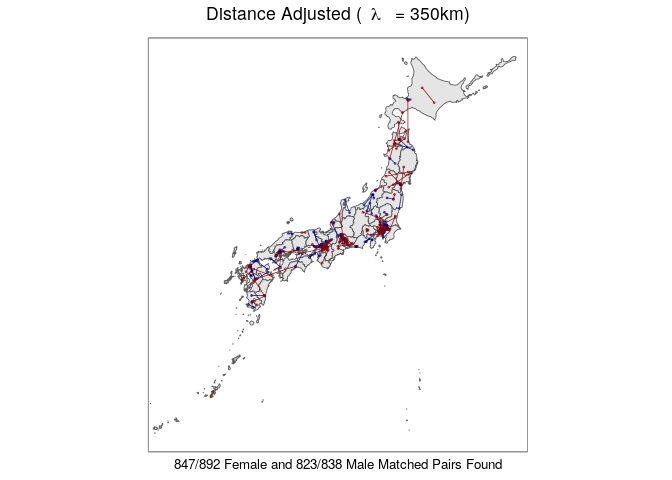
\includegraphics{visualization_2_matching_v5_files/figure-latex/unnamed-chunk-6-5.pdf}

\hypertarget{export-map-plots}{%
\subsection{Export Map Plots}\label{export-map-plots}}

\begin{Shaded}
\begin{Highlighting}[]
\NormalTok{foottxt <-}\StringTok{ }\KeywordTok{paste0}\NormalTok{(}\StringTok{"Dots represent randomly sampled "}\NormalTok{, N, }\StringTok{" matched respondent pairs"}\NormalTok{,}
                  \StringTok{" and lines connect two matched pairs "}\NormalTok{,}
                  \StringTok{"on the map (red = female, }\CharTok{\textbackslash{}n}\StringTok{blue = male). The left panel shows the matching outcome "}\NormalTok{,}
                  \StringTok{"without geographic distance adjustment and "}\NormalTok{,}
                  \StringTok{"the right panel shows }\CharTok{\textbackslash{}n}\StringTok{the outcome of matching with geographic distance adjustment."}\NormalTok{)}

\NormalTok{p <-}\StringTok{ }\KeywordTok{arrangeGrob}\NormalTok{(p1,p2, }\DataTypeTok{nrow=}\DecValTok{1}\NormalTok{,}
                 \DataTypeTok{bottom=}\KeywordTok{textGrob}\NormalTok{(foottxt, }\DataTypeTok{vjust=}\FloatTok{0.5}\NormalTok{,}\DataTypeTok{just=}\StringTok{"left"}\NormalTok{,}\DataTypeTok{x=}\KeywordTok{unit}\NormalTok{(}\FloatTok{0.05}\NormalTok{,}\StringTok{"npc"}\NormalTok{),}
                                 \DataTypeTok{gp=}\KeywordTok{gpar}\NormalTok{(}\DataTypeTok{fontsize=}\DecValTok{9}\NormalTok{)))}
\KeywordTok{grid.arrange}\NormalTok{(p)}
\end{Highlighting}
\end{Shaded}

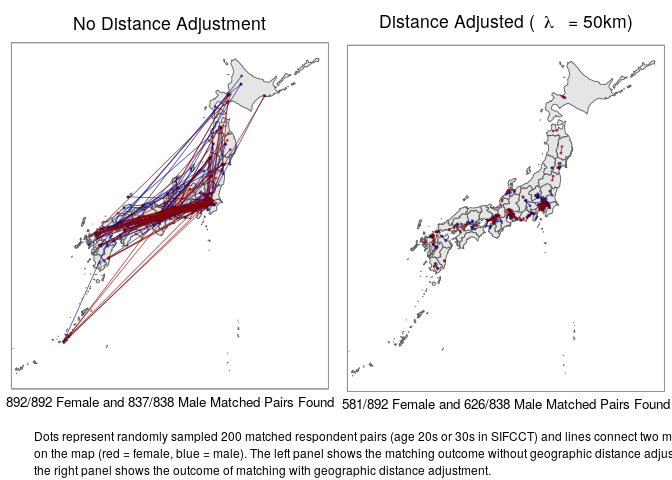
\includegraphics{visualization_2_matching_v5_files/figure-latex/unnamed-chunk-7-1.pdf}

\begin{Shaded}
\begin{Highlighting}[]
\KeywordTok{ggsave}\NormalTok{(}\KeywordTok{paste0}\NormalTok{(projdir,}\StringTok{"/out/geomatchplot_l50_sifcct_v5.pdf"}\NormalTok{),p,}\DataTypeTok{width=}\DecValTok{8}\NormalTok{,}\DataTypeTok{height=}\DecValTok{5}\NormalTok{)}
\end{Highlighting}
\end{Shaded}

\begin{Shaded}
\begin{Highlighting}[]
\NormalTok{p <-}\StringTok{ }\KeywordTok{arrangeGrob}\NormalTok{(p1,p3, }\DataTypeTok{nrow=}\DecValTok{1}\NormalTok{,}
                 \DataTypeTok{bottom=}\KeywordTok{textGrob}\NormalTok{(foottxt,}
                                 \DataTypeTok{vjust=}\FloatTok{0.5}\NormalTok{,}\DataTypeTok{just=}\StringTok{"left"}\NormalTok{,}\DataTypeTok{x=}\KeywordTok{unit}\NormalTok{(}\FloatTok{0.05}\NormalTok{,}\StringTok{"npc"}\NormalTok{),}
                                 \DataTypeTok{gp=}\KeywordTok{gpar}\NormalTok{(}\DataTypeTok{fontsize=}\DecValTok{9}\NormalTok{)))}
\KeywordTok{grid.arrange}\NormalTok{(p)}
\end{Highlighting}
\end{Shaded}

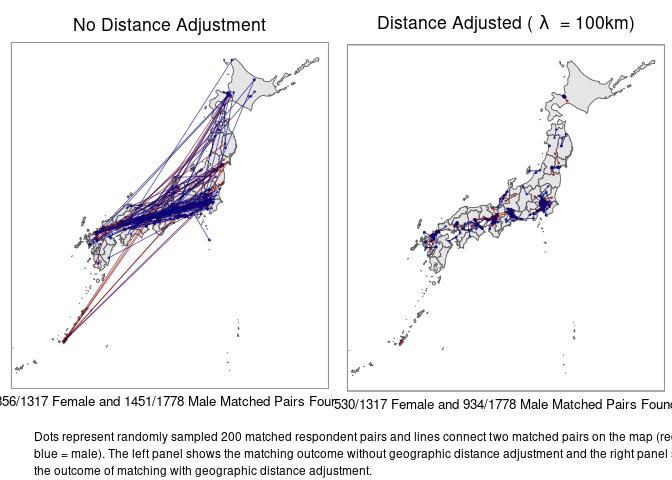
\includegraphics{visualization_2_matching_v5_files/figure-latex/unnamed-chunk-9-1.pdf}

\begin{Shaded}
\begin{Highlighting}[]
\KeywordTok{ggsave}\NormalTok{(}\KeywordTok{paste0}\NormalTok{(projdir,}\StringTok{"/out/geomatchplot_l100_sifcct_v5.pdf"}\NormalTok{),p,}\DataTypeTok{width=}\DecValTok{8}\NormalTok{,}\DataTypeTok{height=}\DecValTok{5}\NormalTok{)}
\end{Highlighting}
\end{Shaded}

\begin{Shaded}
\begin{Highlighting}[]
\NormalTok{p <-}\StringTok{ }\KeywordTok{arrangeGrob}\NormalTok{(p1,p4, }\DataTypeTok{nrow=}\DecValTok{1}\NormalTok{,}
                 \DataTypeTok{bottom=}\KeywordTok{textGrob}\NormalTok{(foottxt, }\DataTypeTok{vjust=}\FloatTok{0.5}\NormalTok{,}\DataTypeTok{just=}\StringTok{"left"}\NormalTok{,}\DataTypeTok{x=}\KeywordTok{unit}\NormalTok{(}\FloatTok{0.05}\NormalTok{,}\StringTok{"npc"}\NormalTok{),}
                                 \DataTypeTok{gp=}\KeywordTok{gpar}\NormalTok{(}\DataTypeTok{fontsize=}\DecValTok{9}\NormalTok{)))}
\KeywordTok{grid.arrange}\NormalTok{(p)}
\end{Highlighting}
\end{Shaded}

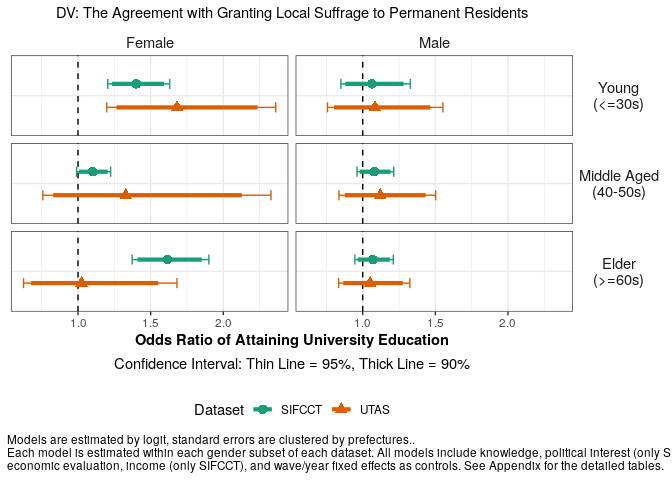
\includegraphics{visualization_2_matching_v5_files/figure-latex/unnamed-chunk-11-1.pdf}

\begin{Shaded}
\begin{Highlighting}[]
\KeywordTok{ggsave}\NormalTok{(}\KeywordTok{paste0}\NormalTok{(projdir,}\StringTok{"/out/geomatchplot_l200_sifcct_v5.pdf"}\NormalTok{),p,}\DataTypeTok{width=}\DecValTok{8}\NormalTok{,}\DataTypeTok{height=}\DecValTok{5}\NormalTok{)}
\end{Highlighting}
\end{Shaded}

\begin{Shaded}
\begin{Highlighting}[]
\NormalTok{p <-}\StringTok{ }\KeywordTok{arrangeGrob}\NormalTok{(p1,p5, }\DataTypeTok{nrow=}\DecValTok{1}\NormalTok{,}
                 \DataTypeTok{bottom=}\KeywordTok{textGrob}\NormalTok{(foottxt, }\DataTypeTok{vjust=}\FloatTok{0.5}\NormalTok{,}\DataTypeTok{just=}\StringTok{"left"}\NormalTok{,}\DataTypeTok{x=}\KeywordTok{unit}\NormalTok{(}\FloatTok{0.05}\NormalTok{,}\StringTok{"npc"}\NormalTok{),}
                                 \DataTypeTok{gp=}\KeywordTok{gpar}\NormalTok{(}\DataTypeTok{fontsize=}\DecValTok{9}\NormalTok{)))}
\KeywordTok{grid.arrange}\NormalTok{(p)}
\end{Highlighting}
\end{Shaded}

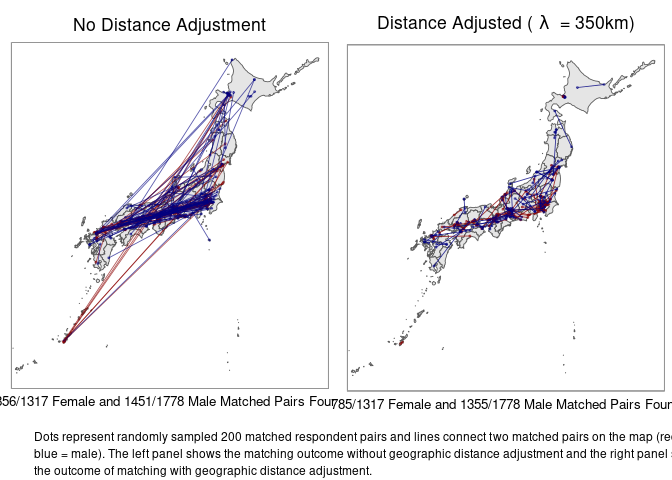
\includegraphics{visualization_2_matching_v5_files/figure-latex/unnamed-chunk-13-1.pdf}

\begin{Shaded}
\begin{Highlighting}[]
\KeywordTok{ggsave}\NormalTok{(}\KeywordTok{paste0}\NormalTok{(projdir,}\StringTok{"/out/geomatchplot_l350_sifcct_v5.pdf"}\NormalTok{),p,}\DataTypeTok{width=}\DecValTok{8}\NormalTok{,}\DataTypeTok{height=}\DecValTok{5}\NormalTok{)}
\end{Highlighting}
\end{Shaded}

\end{document}
